\subsection{表面元素}

本节中，令 q 表示包含于 A 的根基中的一个理想，并令 M 为非零有限生成 A-模，使得 M/qM 具有有限长度。

命题 8. --- 令 \(\delta > 0\) 为一个整数，\(x\) 为 \(\mathfrak{q}^{\delta}\) 中的元素，\(\xi\) 为它在 \(\mathrm{gr}_{\delta}(\mathbf{A}) = \mathfrak{q}^{\delta}/\mathfrak{q}^{\delta+1}\) 中的类，并令 \(\varphi\) 表示 \(\xi\) 在 \(\mathrm{gr}(\mathbf{A})\)-模 \(\mathrm{gr}(\mathbf{M})\) 上的乘法作用。

\begin{enumerate}
\def\labelenumi{\alph{enumi})}
\item
  A-模 M/xM 的维数等于 \(\dim_{\mathbf{A}}(\mathbf{M})\) 或 \(\dim_{\mathbf{A}}(\mathbf{M}) - 1\)。在第二种情形下，有 \(e_{\mathfrak{q}}(\mathbf{M}/x\mathbf{M}) \geqslant \delta e_{\mathfrak{q}}(\mathbf{M})\)。
\item
  假设 \(\dim_{\mathbf{A}}(\mathbf{M}) \geqslant 1\)，并且 \(\varphi\) 的核作为 A/q-模具有有限长度。则有 \(\dim_{\mathbf{A}}(\mathbf{M}/x\mathbf{M}) = \dim_{\mathbf{A}}(\mathbf{M}) - 1\)。此外：
\end{enumerate}

\begin{enumerate}
\def\labelenumi{(\roman{enumi})}
\item
  若 \(\dim_{\mathbf{A}}(\mathbf{M}) > 1\)，则有 \(e_{\mathfrak{q}}(\mathbf{M} / x\mathbf{M}) = \delta e_{\mathfrak{q}}(\mathbf{M})\)。
\item
  若 \(\dim_{\mathbf{A}}(\mathbf{M}) = 1\)，则对每个整数 \(n \geqslant 0\)，有
\end{enumerate}

\[
n \delta e _ {\mathfrak {q}} (\mathrm{M}) \leqslant \operatorname{long} _ {\mathrm{A}} (\mathrm{M} / x ^ {n} \mathrm{M}) \leqslant n \delta e _ {\mathfrak {q}} (\mathrm{M}) + \operatorname{long} _ {\mathrm{A} / \mathfrak {q}} (\operatorname{Ker} \varphi^ {n}),
\]

其中 \(\varphi^n\) 是第 \(n\) 次自同态 \(\varphi\) 的迭代，并且

\[
\delta e _ {\mathfrak {q}} (\mathbf {M}) = e _ {x \mathbf {A}} (\mathbf {M}) \leqslant \operatorname{long} _ {\mathbf {A}} (\mathbf {M} / x \mathbf {M}).
\]

置 \(\mathbf{M}'' = \mathbf{M} / x\mathbf{M}\)；考察 Hilbert-Samuel 级数 \(\mathbf{H}_{\mathbf{M}} = \mathbf{H}_{\mathbf{M},\mathfrak{q}}\) 和 \(\mathbf{H}_{\mathbf{M}''} = \mathbf{H}_{\mathbf{M}'',\mathfrak{q}}\)，以及 Poincaré 级数 \(\mathbf{P}(\mathbf{T}) = \sum_{n\geqslant 0}\mathrm{long}_{\mathbf{A} / \mathfrak{q}}(\mathrm{Ker}\varphi_n)\mathbf{T}^n\)。根据第 4 节第 3 号定理 2 和第 4 号备注 2，有

\[
\mathrm{H} _ {\mathbf {M}} (\mathrm{T}) = (1 - \mathrm{T}) ^ {- d} \mathrm{R} _ {\mathbf {M}} (\mathrm{T}), \quad \mathrm{H} _ {\mathbf {M} ^ {\prime \prime}} (\mathrm{T}) = (1 - \mathrm{T}) ^ {- d ^ {\prime \prime}} \mathrm{R} _ {\mathbf {M} ^ {\prime \prime}} (\mathrm{T}),
\]

其中 \(d = \dim_{\mathbf{A}}(\mathbf{M})\)，\(d'' = \dim_{\mathbf{A}}(\mathbf{M}'')\)，\(\mathbf{R}_{\mathbf{M}}\) 和 \(\mathbf{R}_{\mathbf{M}''}\) 属于 \(\mathbf{Z}[T]\)，\(\mathbf{R}_{\mathbf{M}}(1) = e_{\mathfrak{q}}(\mathbf{M})\)，\(\mathbf{R}_{\mathbf{M}''}(1) = e_{\mathfrak{q}}(\mathbf{M}'')\)。由第 4 节第 5 号引理 6，在 \(\mathbf{Z}((T))\) 中有不等式

\[
\left(1 - \mathrm{T} ^ {\delta}\right) \mathrm{H} _ {\mathbf {M}} ^ {(1)} \leqslant \mathrm{H} _ {\mathbf {M} ^ {\prime \prime}} ^ {(1)} \leqslant \left(1 - \mathrm{T} ^ {\delta}\right) \mathrm{H} _ {\mathbf {M}} ^ {(1)} + \mathrm{T} ^ {\delta} \mathrm{P} ^ {(1)}.
\]

令 \(\mathrm{R}(\mathrm{T}) = (1 - \mathrm{T}^{\delta}) / (1 - \mathrm{T}) = 1 + \mathrm{T} + \cdots + \mathrm{T}^{\delta-1},\) 此式也可写成

\[
\begin{array}{r l} (1) & (1 - \mathrm{T}) ^ {- d} \mathrm{R(T)} \mathrm {R_ {M} (T)} \leqslant (1 - \mathrm{T}) ^ {- d ^ {\prime \prime} - 1} \mathrm {R_ {M^ {\prime\prime}} (T)} \leqslant \\ & \leqslant (1 - \mathrm{T}) ^ {- d} \mathrm{R(T)} \mathrm {R_ {M} (T)} + (1 - \mathrm{T}) ^ {- 1} \symrm {T^ {\delta} P(T)}. \end{array}
\]

由第 4 节第 1 号引理 2，第一条不等式 (1) 蕴含：要么 \(d'' \geqslant d\)，要么 \(d'' = d - 1\) 且 R(1) R \(_{M}\) (1) \(\leqslant\) R \(_{M''}\) (1)，即 \(\delta e_{\mathfrak{q}}(\mathbf{M}) \leqslant e_{\mathfrak{q}}(\mathbf{M}'')\)。这证明了 \(a\) )，因为 \(d'' \leqslant d\)。

在 \(b\) ) 的假设下，有 \(\mathbf{P}(\mathbf{T}) \in \mathbf{Z}[\mathbf{T}]\) 且 \(\mathbf{P}(1) = \text{long}_{\mathbf{A}}(\text{Ker } \varphi)\)。第二个不等式 (1) 写作

\[
(1 - \mathrm{T}) ^ {- d ^ {\prime \prime} - 1} \mathrm{R} _ {\mathrm{M} ^ {\prime \prime}} (\mathrm{T}) \leqslant (1 - \mathrm{T}) ^ {- d} \left(\mathrm{R} (\mathrm{T}) \mathrm{R} _ {\mathrm{M}} (\mathrm{T}) + \mathrm{T} ^ {\delta} (1 - \mathrm{T}) ^ {d - 1} \mathrm{P} (\mathrm{T})\right).
\]

设 \(d > 1\)；则第 4 节第 1 号引理 2 蕴含 \(d'' + 1 \leqslant d\)，因而 \(d'' = d - 1\)，这是根据证明中的 \(a\) ) 部分得到的；于是有

\[
\mathrm{R} _ {\mathbf {M} ^ {\prime \prime}} (1) \leqslant \mathrm{R} (1)\cdot \mathrm{R} _ {\mathbf {M}} (1)
\]

(同上)，从而得到 (i)。

现在设 \(d=1\)。由同上，有 \(d''=0\)，并且

\[
\mathrm{R} _ {\mathbf {M} ^ {\prime \prime}} (1) \leqslant \mathrm{R} (1)\cdot \mathrm{R} _ {\mathbf {M}} (1) + \mathrm{P} (1).
\]

因此，\(\mathbf{M}''\) 具有有限长度，且其长度等于 \(e_{\mathfrak{q}}(\mathbf{M}^{\prime \prime}) = \mathbf{R}_{\mathbf{M}''}(1)\)，从而得到

\[
\delta e _ {\mathfrak {q}} (\mathrm{M}) \leqslant \operatorname{long} _ {\mathrm{A}} (\mathrm{M} / x \mathrm{M}) \leqslant \delta e _ {\mathfrak {q}} (\mathrm{M}) + \operatorname{long} _ {\mathrm{A}} (\operatorname{Ker} \varphi).\tag{2}
\]

令 \(n \geqslant 1\) 为一个整数。在 (2) 中将 \(x\) 替换为 \(x^n\)；于是有

\[
n \delta e _ {\mathfrak{q}} (\mathbf {M}) \leqslant \operatorname{long} _ {\mathbf {A}} (\mathbf {M} / x ^ {n} \mathbf {M}) \leqslant n \delta e _ {\mathfrak{q}} (\mathbf {M}) + \operatorname{long} _ {\mathbf {A}} (\operatorname{Ker} \varphi^ {n}).\tag{3}
\]

显然，诺特 gr(A)-模 gr(M) 的子模 Ker \(\varphi^{n}\) 构成递增序列，因而最终稳定，并且每个子模作为 A/q-模都具有有限长度。将不等式 (3) 除以 \(n \geqslant 1\)，并令 \(n\) 趋于 \(+\infty\)，从而得到 \(e_{xA}(M) = \delta e_{\mathfrak{q}}(\mathbf{M})\)，这是 \(e_{xA}(M)\) 的定义。

引理 3. — 令 R 为次数 ≥ 0 的分次诺特环，E 为有限生成分次 R-模，并满足 \(E_{n}\) 是有限长度的 \(R_{0}\)-模，且这一点对每个 \(n \in Z\) 都成立。以下条件等价：

\begin{enumerate}
\def\labelenumi{(\roman{enumi})}
\item
  E 是具有有限长度的 R-模；
\item
   存在整数 \(n_0\)，使得 \(\mathrm{E}_n = 0\) 对所有 \(n \geqslant n_0\) 都成立；
\item
  \(\mathbf{R}\) 的每个与 \(\mathbf{E}\) 相关的素理想都包含 \(\mathbf{R}_{+} = \bigoplus_{n\geqslant 1}\mathbf{R}_{n}\)。
\item
  \((i) \Leftrightarrow (ii)\)：这是显然的。
\item
  \((iii) \Rightarrow (i)\)：令 \(p\) 为一个与 E 相关的素理想。若满足 (iii)，则有 \(p = p_0 + R_+\)，其中 \(p_0\) 是 \(R_0\) 的素理想，且 R-模 \(R/p\) 同构于 \(R_0/p_0\)。根据 IV, § 3, n° 1, 命题 1 的推论，\(R_0\)-模 \(R_0/p_0\) 同构于某个 \(E_k\) 的子模，因而具有有限长度。因此 R/p 具有有限长度。根据 IV, § 2, n° 5, 命题 7，p 因而是极大理想。由于 p 任意，R-模 E 具有有限长度（同上）。
\item
  \((i) \Rightarrow (iii)\)：令 \(p\) 为一个与 E 相关的素理想。则 \(p\) 是分次的（IV, § 3, 第 1 号, 命题 1）且是极大的（IV, § 2, 第 5 号, 命题 7），因而包含 \(R_{+}\)（§ 6, 第 2 号, 引理 1）。
\end{enumerate}

命题 9. --- 记 \(\mathfrak{p}_1, \ldots, \mathfrak{p}_r\) 为分次环 \(\mathrm{gr}(\mathrm{A}) = \bigoplus_{n} (\mathfrak{q}^n / \mathfrak{q}^{n+1})\) 的素理想中那些与分次模 \(\mathrm{gr}(\mathrm{M}) = \bigoplus_{n} (\mathfrak{q}^n \mathrm{M} / \mathfrak{q}^{n+1} \mathrm{M})\) 相关且不包含 \(\mathrm{gr}_1(\mathrm{A}) = \mathfrak{q} / \mathfrak{q}^2\) 的素理想。令 \(\delta\) 为整数 \(>0\)，\(\xi\) 为 \(\mathrm{gr}_{\delta}(\mathrm{A})\) 中的元素，并令 \(\varphi : \mathrm{gr}(\mathrm{M}) \to \mathrm{gr}(\mathrm{M})\) 表示比值为 \(\xi\) 的 \(\mathrm{gr}(\mathrm{M})\) 上的伸缩。映射 \(\varphi_n\) 对所有充分大的 \(n\) 都是单射，当且仅当 \(\xi^n\) 不属于任何 \(\mathfrak{p}_i\)。

事实上，gr(A)-模 Ker φ 的相关素理想正是 gr(M) 的相关素理想中包含 ξ 的那些（IV, § 1, 第 1 号, 定义 1）。根据引理 3，(Ker φ) \(_n\) 在 \(n\) 足够大时为零，当且仅当这些理想都包含 \(\mathrm{gr}_{+}(\mathrm{A})\)（或等价地，包含 \(\mathrm{gr}_{1}(\mathrm{A})\)），命题得证。

定义 2. --- 令 A 为诺特环，q 为包含于 A 的根基中的 A-理想，并令 M 为有限生成 A-模，使得 M/qM 具有有限长度。如果 x 属于 q，且对所有充分大的 n，由 x 的乘法所诱导的映射 \(\mathfrak{q}^{n}\mathbf{M}/\mathfrak{q}^{n+1}\mathbf{M} \to \mathfrak{q}^{n+1}\mathbf{M}/\mathfrak{q}^{n+2}\mathbf{M}\) 是单射，则称 A 的元素 x 关于 q 对 M 是表面元素。

备注。--- 1) 令 δ 为一个 \textgreater{} 0 的整数。若 \(x \in \mathfrak{q}^{\delta}\)，且对所有充分大的 n，由 x 的乘法所诱导的映射 \(\mathfrak{q}^{n}\mathbf{M}/\mathfrak{q}^{n+1}\mathbf{M} \to \mathfrak{q}^{n+\delta}\mathbf{M}/\mathfrak{q}^{n+\delta+1}\mathbf{M}\) 是单射，有时称 A 的元素 x 关于 q 对 M 是阶数为 δ 的表面元素。按此术语，定义 2 意义下的表面元素就是阶数为 1 的表面元素。

\begin{enumerate}
\def\labelenumi{\arabic{enumi})}
\setcounter{enumi}{1}
\item
   采用命题 9 的记号，\(x\) 是阶数为 \(\delta\) 的表面元素，当且仅当它的类 \(\xi\) 在 \(\mathrm{gr}_{\delta}(\mathbf{A})\) 中不属于任何一个 \(\mathfrak{p}_i\)。
\item
  根据 III, § 1, 第 4 号, 命题 8，存在一个 \(\mathrm{gr}(\mathrm{A})\) 中次数为 \(>0\) 且不属于任何一个 \(\mathfrak{p}_i\) 的齐次元素。因此，存在整数 \(\delta > 0\) 以及一个对 M 阶数为 \(\delta\) 的表面元素。
\item
   假设 A 是局部环，剩余域为 \(k\)，并考察典范满射 \(\lambda: \mathfrak{q} \to \mathfrak{q} \otimes_{\mathbf{A}} k\)。它是典范映射 \(\mathfrak{q} \to \mathfrak{q}/\mathfrak{q}^2\) 与 \(\overline{\lambda}: \mathfrak{q}/\mathfrak{q}^2 \to \mathfrak{q} \otimes_{\mathbf{A}} k\) 的复合。根据 Nakayama 引理，\(V_i = \overline{\lambda}(\mathfrak{p}_i \cap (\mathfrak{q}/\mathfrak{q}^2))\) 是 \(\mathfrak{q} \otimes_{\mathbf{A}} k\) 的向量子空间，且上述各空间都不等于 \(\mathfrak{q} \otimes_{\mathbf{A}} k\)；若 \(\alpha \in \mathfrak{q} \otimes_{\mathbf{A}} k\) 不属于任何一个 \(V_i\)，则 \(\lambda^{-1}(\alpha)\) 中的元素都是对 M 的表面元素（命题 9）。若 \(k\) 是无限域，则 \(V_i\) 的并集不等于 \(\mathfrak{q} \otimes_{\mathbf{A}} k\)，因而存在对 M 的表面元素。
\end{enumerate}

定理 1. --- 令 A 为诺特环，q 为包含于 A 的根基中的 A-理想，并令 M 为有限生成 A-模，使得 M/qM 具有有限长度。令 \(x_{1}, \ldots, x_{m}\) 为 q 中元素的有限序列。置 \(x = Ax_{1} + \cdots + Ax_{m} \subset q\)。

\begin{enumerate}
\def\labelenumi{\alph{enumi})}
\item
  有 \(\dim_{\mathbf{A}}(\mathbf{M} / \mathfrak{x}\mathbf{M})\geqslant \dim_{\mathbf{A}}(\mathbf{M}) - m.\)
\item
  若 \(\dim_{\mathbf{A}}(\mathbf{M} / \mathfrak{x}\mathbf{M}) = \dim_{\mathbf{A}}(\mathbf{M}) - m\)，则 \(e_{\mathfrak{q}}(\mathbf{M} / \mathfrak{x}\mathbf{M}) \geqslant e_{\mathfrak{q}}(\mathbf{M})\)。
\item
  若 \(m < \dim_{\mathbf{A}}(\mathbf{M})\)，且对于 \(i = 1, \ldots, m\)，A 的元素 \(x_{i}\) 关于 q 对 \(\mathbf{M}/(x_{1}\mathbf{M} + \cdots + x_{i-1}\mathbf{M})\) 是表面元素，则有
\end{enumerate}

\[
\dim_{\mathbf{A}}(\mathbf{M} / \mathfrak{x}\mathbf{M}) = \dim_{\mathbf{A}}(\mathbf{M}) - m \quad\text{且}\quad e_{\mathfrak{q}}(\mathbf{M} / \mathfrak{x}\mathbf{M}) = e_{\mathfrak{q}}(\mathbf{M}).
\]

\begin{enumerate}
\def\labelenumi{\alph{enumi})}
\setcounter{enumi}{3}
\tightlist
\item
  若 \(m = \dim_{\mathbf{A}}(\mathbf{M})\)，且对于 \(i = 1, \ldots, m\)，A 的元素 \(x_{i}\) 关于 q 对 \(\mathbf{M}/(x_{1}\mathbf{M} + \cdots + x_{i-1}\mathbf{M})\) 是表面元素，则有
\end{enumerate}

\[
e _ {\mathfrak {q}} (\mathbf {M}) = e _ {\mathfrak {x}} (\mathbf {M}) \leqslant \operatorname{long} (\mathbf {M} / \mathfrak{x}\mathbf{M}) <   + \infty .
\]

当 \(a\) )、\(b\) ) 和 \(c\) ) 在 \(m = 1\) 时由命题 8 得出，一般情形则由归纳法得到。假设 \(d\) ) 的假设成立，并置 \(\mathbf{x}' = \mathrm{A}x_{1} + \cdots + \mathrm{A}x_{m-1}\) 与 \(\mathbf{M}' = \mathbf{M}/\mathbf{x}'\mathbf{M}\)，从而 \(\mathbf{M}/\mathbf{x}\mathbf{M}\) 可识别为 \(\mathbf{M}'/x_{m}\mathbf{M}'\)。于是根据 \(c\) )，有 \(\dim_{\mathbf{A}}(\mathbf{M}') = 1\) 且 \(e_{\mathfrak{q}}(\mathbf{M}) = e_{\mathfrak{q}}(\mathbf{M}')\)。由命题 8，\(\mathbf{M}/\mathbf{x}\mathbf{M}\) 具有有限长度，且 \(e_{\mathfrak{q}}(\mathbf{M}') = e_{x_{m}\mathbf{A}}(\mathbf{M}') \leqslant \text{long}(\mathbf{M}/\mathbf{x}\mathbf{M})\)。但是，由于 \(x_{m}^{n}\mathbf{M}' = \mathfrak{x}^{n}\mathbf{M}'\) 对每个 \(n\) 都成立，故 \(e_{x_{m}\mathbf{A}}(\mathbf{M}') = e_{\mathfrak{x}}(\mathbf{M}')\)。另一方面，有 \(e_{\mathfrak{x}}(\mathbf{M}') \geqslant e_{\mathfrak{x}}(\mathbf{M})\)；这是由 \(b\) ) 得出的，其中将 \(m\) 替换为 \(m - 1\)，将 \(x\) 替换为 \(x'\)，并将 \(q\) 替换为 \(\mathfrak{x}\)。因此，有

\[
e _ {\mathfrak {x}} (\mathrm{M}) \leqslant e _ {\mathfrak {x}} (\mathrm{M} ^ {\prime}) = e _ {x _ {m} \mathrm{A}} (\mathrm{M} ^ {\prime}) = e _ {\mathfrak {q}} (\mathrm{M} ^ {\prime}) = e _ {\mathfrak {q}} (\mathrm{M}).
\]

由于 \(\mathfrak{x}\) 包含于 \(\mathfrak{q}\)，这意味着 \(e_{\mathfrak{x}}(\mathbf{M}) = e_{\mathfrak{q}}(\mathbf{M})\)（第 1 号, 备注 1），证明完成。

推论。--- 假设 A 是局部环且剩余域无限，并令 \(d = \dim_{\mathbf{A}}(\mathbf{M})\)。存在 q 中元素的序列 \(x_{1}, \ldots, x_{d}\)，使得置 \(x = Ax_{1} + \cdots + Ax_{d}\) 后，有

\[
e _ {\mathfrak {q}} (\mathbf {M}) = e _ {\mathfrak {x}} (\mathbf {M}) \leqslant \operatorname{long} (\mathbf {M} / \mathfrak{x}\mathbf{M}) <   + \infty .
\]

这立即由定理和备注 4 得出。

备注 5. --- 在前述推论的情形下，有

\[
e _ {\mathfrak {q}} (\mathrm{M}) = e _ {\mathfrak {x}} (\mathrm{M}) \leqslant \operatorname{long} (\mathrm{M} / \mathfrak {x} \mathrm{M})
\]

\pandocbounded{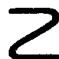
\includegraphics[keepaspectratio]{images/part001_8adf5445.jpg}}

并且 \(\operatorname{long}(\mathbf{M} / \mathfrak{q}\mathbf{M})\leqslant \operatorname{long}(\mathbf{M} / \mathfrak{x}\mathbf{M})\)；以下三种情形

\[
e _ {\mathfrak {q}} (\mathrm{M}) <   \operatorname{long} (\mathrm{M} / \mathfrak {q} \mathrm{M}), e _ {\mathfrak {q}} (\mathrm{M}) = \operatorname{long} (\mathrm{M} / \mathfrak {q} \mathrm{M}), e _ {\mathfrak {q}} (\mathrm{M}) > \operatorname{long} (\mathrm{M} / \mathfrak {q} \mathrm{M})
\]

是可能的（第~106页，习题 16 和 17）。

\specialchapter{习题}
\setcounter{exercisesection}{0}

\exercisesection{环的克鲁尔维数}

\begin{enumerate}
\def\labelenumi{\arabic{enumi})}
\tightlist
\item
  令 X 为拓扑空间，Y 为 X 的子空间。若对于 X 的每个闭子集 F，F 都是 F ∩ Y 的闭包，则称 Y 在 X 中非常稠密。
\end{enumerate}

\begin{enumerate}
\def\labelenumi{\alph{enumi})}
\item
  Y 在 X 中非常稠密的必要且充分条件是：对于 X 的每个非空局部闭子集 F，F ∩ Y 非空。
\item
  若 Y 在 X 中非常稠密，且 Z 是 Y 的在 X 中非常稠密的子空间，则 Z 在 X 中非常稠密。若 Y 在 X 中非常稠密，且 F 是 X 的局部闭子集，则 Y ∩ F 在 F 中非常稠密。
\item
  若 Y 在 X 中非常稠密，则有 \(\dim(\mathbf{Y}) = \dim(\mathbf{X})\)。
\end{enumerate}

\begin{enumerate}
\def\labelenumi{\arabic{enumi})}
\setcounter{enumi}{1}
\item
  令 A 为环，Specmax(A) 为 A 的极大理想集合。Specmax(A) 在 Spec(A) 中非常稠密的充要条件是 A 为 Jacobson 环（V, § 3, 第 4 号）。此时有 dim Specmax(A) = dim(A)。
\item
  证明：若 A 是 Jacobson 环，则 A{[}{[}X{]}{]} 不是 Jacobson 环。（比较 Specmax(A) 与 Specmax(A{[}{[}X{]}{]})。）
\item
  \begin{enumerate}
  \def\labelenumii{\alph{enumii})}
  \tightlist
  \item
    证明：可以唯一地给每个有序集 E 关联一个 \(\{-\infty\}\cup\mathbf{N}\cup\{+\infty\}\) 中的元素，记为 dev(E)（E 的偏差），使其满足下列性质：
  \end{enumerate}
\end{enumerate}

\(\alpha)\) 有 \(\operatorname{dev}(\mathbf{E}) = -\infty\)，当且仅当关系 \(a \leqslant b\) 在 \(\mathbf{E}\) 中蕴含 \(a = b\)。

β) 令 n 为正整数。E 的偏差 ≤ n，当且仅当对于 E 中元素的每个无限递减序列 \((a_{k})_{k\in\mathbb{N}}\)，当 k 充分大时都有 \(\text{dev}([a_{k}, a_{k-1}]) \leqslant n - 1\)。

\begin{enumerate}
\def\labelenumi{\alph{enumi})}
\setcounter{enumi}{1}
\item
  要有 \(\text{dev}(\mathbf{E}) \leqslant 0\)，必要且充分的是 E 中元素的每个严格递减序列都最终稳定。有 \(\text{dev}(\mathbf{N}) = 0\)，\(\text{dev}(\mathbf{Z}) = 1\)，\(\text{dev}(\mathbf{Q}) = +\infty\)。
\item
  若 E 和 F 是有序集，且 \(f: \mathbf{E} \to \mathbf{F}\) 是严格递增映射，则有 \(\operatorname{dev}(\mathbf{E}) \leqslant \operatorname{dev}(\mathbf{F})\)。并且有 \(\operatorname{dev}(\mathbf{E} \times \mathbf{F}) = \sup(\operatorname{dev}(\mathbf{E}), \operatorname{dev}(\mathbf{F}))\)。
\item
  令 S(E) 为 E 中元素的无限递增稳定序列集合，并按积序排序。则有 \(\operatorname{dev}(\mathbf{S}(\mathbf{E})) = \operatorname{dev}(\mathbf{E}) + 1\)。
\end{enumerate}

\begin{enumerate}
\def\labelenumi{\arabic{enumi})}
\setcounter{enumi}{4}
\tightlist
\item
  若 A 是环（不必交换），M 是左 A-模，则以 Kdev(M) 表示按包含关系排序的 M 的子模集合的偏差。规定 \(Kdev(A) = Kdev(A_s)\)。
\end{enumerate}

\begin{enumerate}
\def\labelenumi{\alph{enumi})}
\tightlist
\item
  若 N 是 A-模 M 的子模，则有
\end{enumerate}

\[
\operatorname{Kdev} (\mathbf {M}) = \sup (\operatorname{Kdev} (\mathbf {N}), \operatorname{Kdev} (\mathbf {M} / \mathbf {N}))  .
\]

\begin{enumerate}
\def\labelenumi{\alph{enumi})}
\setcounter{enumi}{1}
\item
  假设 A 交换。若 p 和 q 是 A 的两个素理想，满足 p ⊂ q 且 p ≠ q，则有 dev(A/p) \textgreater{} dev(A/q)。（使用理想 p + Ax，其中 x 是 q - p 中的元素。）推导出 dim(A) ≤ Kdev(A)。
\item
   假设 A 是交换诺特环。证明 dim(A) = Kdev(A)（对 dim(A) 作归纳，假设对于每个交换诺特环 B，只要 dim(B) \textless{} dim(A) 就有 Kdev(B) ≤ dim(B)；令 S 为 A 中不属于任何满足 dim(A) = dim(A/p) 的 A 的素理想 p 的元素 s 所成的集合；证明：对于每个有限生成 A-模 M，若 \(S^{-1}M = 0\)，则有 \(\mathrm{Kdev}(\bar{\mathrm{M}}) < \dim(\mathrm{A})\)；利用 \(S^{-1}A\) 为 Artin 环这一事实，从而推出 \(\mathrm{Kdev}(\mathrm{A}) \leqslant \dim(\mathrm{A})\)。证明对每个有限生成 A-模 M 都有 \(\dim(\mathrm{M}) = \mathrm{Kdev}(\mathrm{M})\)。
\end{enumerate}

6). a) 令 A 为诺特（交换）环，m 为包含于 A 的根基中的 A-理想，并令 gr(A) 为与 A 的 m-进滤过相关联的分次环。给 A 的每个理想关联 gr(A) 的一个理想，并由此推出 Kdev(A) ≤ Kdev(gr(A))（参见习题 4, c)）。因此有 dim(A) ≤ dim(gr(A))（习题 5, c)）。

\begin{enumerate}
\def\labelenumi{\alph{enumi})}
\setcounter{enumi}{1}
\tightlist
\item
  现在假设 m = xA，其中 x 属于 A 的根基。证明 gr(A) 同构于分次代数 (A/m)[T] 的一个商。证明 (A/m) {[}T{]} 的分次理想有序集 F 同构于 A/m 的递增理想序列集合；由此根据（习题 4, d)）得到 dev(F) = Kdev(A/(x)) + 1，进而 dim(A) ≤ dim(A/m) + 1。
\end{enumerate}

\begin{enumerate}
\def\labelenumi{\arabic{enumi})}
\setcounter{enumi}{6}
\tightlist
\item
  令 A 为 \(C^\infty\) 类函数在 \(\mathbf{R}_{+}\) 上于 0 处的芽环。我们拟证明环 A 的维数无穷。记 C 为 \(C^\infty\) 类函数在 \(\mathbf{R}_{+}\) 上的代数，并令 F 为由在 0 的某个邻域内恒为零的函数组成的理想，从而 \(A = C / F\)。
\end{enumerate}

\begin{enumerate}
\def\labelenumi{\alph{enumi})}
\item
  令 \((x_{n})_{n\in \mathbb{N}}\) 为 \(\mathbf{R}_{+}\) 中严格递减且趋于 0 的序列，并令 \(\mathfrak{U}\) 为 \(\mathbf{N}\) 上比有限集补集滤子更细的超滤子。证明：集合 \(\mathbf{J}_1\) 由满足如下条件的 \(f\in \mathbf{C}\) 组成：对于 \(n\in \mathbf{N}\)，\(f(x_{n}) = 0\) 的那些 n 所成集合属于 \(\mathfrak{U}\)，并且是 \(\mathbf{C}\) 的素理想。
\item
  记 \(\tau_{n}(f)\) 为函数 \(x\mapsto f(x + x_{n})\)。证明：若 J 是 C 的素理想，则集合 \(\varphi(J)\) 由满足以下条件的 \(f\) 组成，并且是 C 的素理想：满足 \(n\in\mathbf{N}\) 且 \(\tau_{n}f\in\mathbf{J}\) 的 n 的集合属于 \(\mathfrak{U}\)。
\item
  定义 C 的理想序列 \(\mathbf{I}_n\)：\(\mathbf{I}_0 = \mathbf{J}_1\)，\(\mathbf{I}_{n+1} = \varphi(\mathbf{I}_n)\)。证明 \((\mathbf{I}_n)_{n\in\mathbb{N}}\) 是包含 F 的 C 的素理想严格递减序列。
\end{enumerate}

\begin{enumerate}
\def\labelenumi{\arabic{enumi})}
\setcounter{enumi}{7}
\item
  令 X 为拓扑空间。证明映射 \(x \mapsto \dim_x(X)\) 从 X 到 \(\overline{\mathbf{R}}\) 是上半连续的。
\item
  令 A 为环，p 为 A 的素理想，M 为有限生成 A-模。证明有：
\end{enumerate}

\[
\dim_ {\mathbf {A} _ {\mathfrak {p}}} (\mathbf {M} _ {\mathfrak {p}}) + \dim_ {\mathbf {A} / \mathfrak {p}} (\mathbf {M} / \mathfrak {p} \mathbf {M}) \leqslant \dim_ {\mathbf {A}} (\mathbf {M}).
\]

\begin{enumerate}
\def\labelenumi{\arabic{enumi})}
\setcounter{enumi}{9}
\tightlist
\item
  如果 Spec(A) 的所有不可约分支都具有相同维数，则称环 A 为等维的。令 A 为环，n 为整数。以下条件等价：
\end{enumerate}

\begin{enumerate}
\def\labelenumi{\alph{enumi})}
\tightlist
\item
  A 的每条素理想链都包含于一条长度为 n 的链中；
\item
  对 A 的每个极大理想 m，环 A \(_{m}\) 都是等维的、串联的，且维数为 n。
\end{enumerate}

\begin{enumerate}
\def\labelenumi{\arabic{enumi})}
\setcounter{enumi}{10}
\tightlist
\item
  令 \((\mathbf{A}_{i}, f_{ij})\) 为相对于滤序集 I 的环的归纳系统，其归纳极限为 A。证明有 \(\dim(\mathbf{A}) \leqslant \lim.\inf\dim(\mathbf{A}_{i})\)，并且当同态 \(f_{ij}\) 忠实平坦时取等号。举一个同态 \(f_{ij}\) 平坦但满足 \(\dim(\mathbf{A}) < \lim.\inf\dim(\mathbf{A}_{i})\) 的例子（取 I = N，\(A_{n} = Z[n^{-1}]\)，A = Q）。
\end{enumerate}

令 A 为环，I 和 J 为 A 的两个理想。假设对 A 的每个极大理想 m，都有 IA \(_{m}\) = JA \(_{m}\)。由此推出 I = J。

\begin{enumerate}
\def\labelenumi{\alph{enumi})}
\setcounter{enumi}{1}
\item
  令 A 为一个环，满足：对 A 的每个极大理想 m，环 \(\mathrm{A}_{\mathfrak{m}}\) 都是诺特环；并且对 A 的每个非零元素 \(f\)，包含 \(f\) 的 A 的极大理想只有有限多个。则 A 是诺特环。（令 \(a\) 为 A 的一个理想。我们首先证明，存在有限族 \((x_1, ..., x_n)\)，其元素属于 \(a\)，使得包含 \(\{x_1, ..., x_n\}\) 的 A 的极大理想都包含 \(a\)。然后我们构造有限族 \(y_1, ..., y_l\) 的元素，使得对 A 的每个极大理想 m，\(\{y_1, ..., y_l\}\) 生成理想 \(a\mathrm{A}_{\mathfrak{m}}\)，该理想属于 \(\mathrm{A}_{\mathfrak{m}}\)。最后使用 a) 得到结论。
\item
  令 A 为半局部环，且对每个极大理想 m，环 \(A_{m}\) 都是诺特环。则 A 是诺特环。
\end{enumerate}

\begin{enumerate}
\def\labelenumi{\arabic{enumi})}
\setcounter{enumi}{12}
\item
  令 K 为域，\((n_{r})_{r\geqslant1}\) 为严格递增且 \textgreater0 的整数序列；对每个整数 \(i\geqslant0\)，记 \(p_{i}\) 为环 \(\mathrm{K}[(\mathrm{X}_{j})_{j\in\mathbb{N}}]\) 中由 \(X_{j}\)（其中 \(n_{1}+\cdots+n_{i}\leqslant j<n_{1}+\cdots+n_{i}+n_{i+1}\)）生成的理想，并令 S 为 \(\mathrm{K}[(\mathrm{X}_{j})]\) 中不属于任何一个 \(p_{i}\) 的元素所成的集合。则环 \(S^{-1}K[(X_{j})]\) 是诺特环且维数无穷（使用习题 12 证明 \(S^{-1}K[(X_{j})]\) 是诺特环）\(^{1}\)。
\item
  令 V 为离散赋值环，令 \(\pi\) 为 V 的一致化元。在环 V{[}T{]} 中，理想 \(m_1 = (\pi T - 1)\) 是高度为 1 的极大理想，理想 \(m_2 = (\pi) + (T)\) 是高度为 2 的极大理想。域 V{[}T{]}/ \(m_1\) 和 V{[}T{]}/ \(m_2\) 分别同构于 V 的分式域和剩余域。有 \(\dim(\mathrm{V}[T]) = 2\)，但 \(\dim(\mathrm{V}[T]/m_1) + \dim(\mathrm{V}[T]_{m_1}) = 1\)，且 \(\dim(\mathrm{gr}_{m_1}(\mathrm{V}[T])) = 1\)。
\end{enumerate}

  沿用前一习题的记号，假设环 V 的剩余域与分式域同构（例如，当 \(\mathrm{V} = k[[\mathrm{U}]]\) 时就是如此，其中域 \(k\) 是带有域中系数的无穷多个不定元形式幂级数环的分式域）。令 \(\sigma\) 为从 \(\mathrm{V[T] / m_1}\) 到 \(\mathrm{V[T] / m_2}\) 的同构。令 C 表示 \(\mathrm{V[T]} = \mathrm{E}\) 的子环，它由 E 中那些模 \(m_1\) 与 \(m_2\) 的类在 \(\sigma\) 下相互对应的元素组成。证明 C 是诺特环，且 \(m_1m_2 = m_1 \cap m_2\) 是 C 的极大理想。证明 E 是 C 的整闭包（注意 \(\mathrm{E} = \mathrm{C} + \mathrm{C}\cdot(\pi T - 1)\)，且 \((\pi T - 1)^2 + (\pi T - 1)\) 属于 C）。

令 \(\mathring{\mathrm{A}}\) 为局部环 \(\mathbf{C}_{\mathfrak{m}_1\mathfrak{m}_2}\)。则 A 是维数为 2 的整环，因而是串联的；\(\mathbf{B} = \mathbf{E} \otimes_{\mathbb{C}} \mathbf{A}\) 是 \(\mathring{\mathrm{A}}\) 的整闭包，是半局部诺特环，恰有两个极大理想 \(\mathfrak{n}_1\) 和 \(\mathfrak{n}_2\)，并且有 \(\dim(\mathbf{B}_{\mathfrak{n}_1}) = 1\)，\(\dim(\mathbf{B}_{\mathfrak{n}_2}) = 2\)。

¶ 16) 沿用前一习题的记号，并将 B 识别为多项式环 A{[}U{]} 对素理想 \(\mathfrak{p}\) 的商，该素理想由 \(U^2 + U - \pi T(\pi T - 1)\) 生成。令 \(\mathfrak{q}_i\) 为 A{[}U{]} 中满足 \(\mathfrak{n}_i = \mathfrak{q}_i/\mathfrak{p}\) 的理想。则 \(\operatorname{ht}(\mathfrak{q}_i) = 3\)，\(\operatorname{ht}(\mathfrak{p}) = 1\)，且链 \(\mathfrak{p} \subset \mathfrak{q}_1\) 是饱和的。特别地，A{[}U{]} 和 A{[}U{]}\(_{\mathfrak{q}_1}\) 不是串联的。

\begin{enumerate}
\def\labelenumi{\arabic{enumi})}
\setcounter{enumi}{16}
\tightlist
\item
  \begin{enumerate}
  \def\labelenumii{\alph{enumii})}
  \tightlist
  \item
    令 A 为整环且 \(f \in \mathrm{A}[\mathrm{T}], f \neq 0\)。证明存在 \(\mathrm{A}[\mathrm{T}]\) 的极大理想 m，使得 \(f \notin \mathfrak{m}\)（取一个包含 T.f-1 的极大理想）。
  \end{enumerate}
\end{enumerate}

\begin{enumerate}
\def\labelenumi{\alph{enumi})}
\setcounter{enumi}{1}
\tightlist
\item
  令 A 为环。证明有 dim(Specmax(A{[}T{]})) \(\geqslant\) dim(A) + 1。（令 \(\mathfrak{p}_0\subset \mathfrak{p}_1\subset \cdots \subset \mathfrak{p}_n\) 为 A 的一条素理想链。考察链
\end{enumerate}

\[
\mathfrak {p} _ {0} [ \mathrm{T} ] \subset \mathfrak {p} _ {1} [ \mathrm{T} ] \subset \mathfrak {p} _ {2} [ \mathrm{T} ] \dots \subset \mathfrak {p} _ {n} [ \mathrm{T} ] \subset (\mathfrak {p} _ {n}, \mathrm{T})
\]

它们是 A{[}T{]} 的素理想，并置

\[
\left\{ \begin{array}{l} \mathrm{U} _ {i} = \mathrm{V} (\mathfrak {p} _ {i} [ \mathrm{T} ]) \cap \operatorname{Specmax} (\mathrm{A} [ \mathrm{T} ]), \quad 0 \leqslant i \leqslant n \\ \mathrm{U} _ {n + 1} = \mathrm{V} (\mathfrak {p} _ {n}, \mathrm{T}) \cap \operatorname{Specmax} (\mathrm{A} [ \mathrm{T} ]). \end{array} \right.
\]

利用 \(a\) ) 证明 \((\mathrm{U}_i)_{0 \leqslant i \leqslant n+1}\) 是 Specmax (A{[}T{]}) 的不可约闭子集严格递增序列。

\begin{enumerate}
\def\labelenumi{\alph{enumi})}
\setcounter{enumi}{2}
\tightlist
\item
  令 \(k\) 为域，并令 S 为由 \(k[\mathrm{X}, \mathrm{Y}]\) 中形如 \(1 + \mathrm{X}g(\mathrm{X}, \mathrm{Y})\) 的元素组成的子集，令 \(\mathrm{A} = \mathrm{S}^{-1}k[\mathrm{X}, \mathrm{Y}]\)。
\end{enumerate}

证明有 dim(Specmax(A)) = 1 且 dim(Spec(A)) = 2。推广到含有多个不定元的情形。

\begin{enumerate}
\def\labelenumi{\alph{enumi})}
\setcounter{enumi}{3}
\item
  证明对于每一对整数 \(0 \leqslant n < m\)，存在诺特环 A，使得 \(\dim(\text{Specmax}(A)) = n\) 且 \(\dim(\text{Specmax}(A[T])) = m\)。
\item
  令 A 为习题 13 中定义的诺特环。证明有 dim(Specmax(A)) = 1 且 dim(Specmax(A{[}T{]})) = \(\infty\)。
\end{enumerate}

\exercisesection{代数的维数}

\begin{enumerate}
\def\labelenumi{\arabic{enumi})}
\item
  令 V 为离散赋值环，分式域为 K，并令 n 为整数。令 A 为多项式环 \(K[X_{1},...,X_{n}]\) 的子环，由常数项属于 V 的多项式组成。由 V 到 A 的典范同态满足性质 (PM)，且典范同态 \(V/m_{V} \rightarrow A/m_{V}A\) 是同构。此外，有 \(\dim(A) \geqslant n + 1\) 且 \(\dim(V) = 1\)。一旦 \(n \geqslant 1\)，因而有 \(\dim(A) > \dim(V) + \dim(A/m_{V}A)\)。证明 A 不是诺特环。利用形式级数，构造一个类似的例子，其中 A 是局部环且不是诺特环。
\item
  令 V 为离散赋值环，分式域为 K，剩余域为 k。记 A 为环 \(K \times k\)，记 \(\rho : V \to A\) 为由 V 到 K 和 k 的典范同态导出的同态。同态 \(\rho\) 是单射，映射 \(^{a}\rho : \text{Spec}(A) \to \text{Spec}(V)\) 是满射，A 是有限生成 V-代数，并且有 \(\dim(A) < \dim(V)\)。
\item
  令 A 为维数为 1 的整环，令 \(\mathfrak{p}_0 \subset \mathfrak{p}_1 \subset \mathfrak{p}_2\) 为 A{[}X{]} 的三个不同的非零素理想。证明有 \(\mathfrak{p}_0 \cap \mathbf{A} = \{0\}\)，\(\mathfrak{p}_1 = (\mathfrak{p}_1 \cap \mathbf{A})\cdot\mathrm{A}{[}X{]}\)，并且 \(\mathfrak{p}_2\) 是 A{[}X{]} 的极大理想。
\item
  令 A 为局部整闭环，\(m_A\) 为其极大理想，K 为其分式域。对于 K 的每个元素 x，记 A{[}x{]} 为 K 中由 x 生成的子 A-代数。令 x 为 K* 中满足 \(x^{-1}\) 不属于 A 的元素。令 A{[}X{]} 为以 A 为系数的单变量 X 多项式环，并令 \(\varphi\) 为取值映射 P \(\mapsto\) P(x)，其定义域为 A{[}X{]}，目标为 A{[}x{]}。
\end{enumerate}

\begin{enumerate}
\def\labelenumi{\alph{enumi})}
\item
  \(\varphi\) 的核是理想 Q，它由形如 \(aX + b\) 的多项式生成，其中 \(a, b \in A\) 且 \(ax + b = 0\)。（若 \(\mathrm{P}(X) = \sum_{i=0}^{n} a_i X^i\) 满足 \(\mathrm{P}(x) = 0\)，注意此时 \(-b_0 = a_0 x\) 在 \(A\) 上整，因而属于 \(A\)。）
\item
  理想 \(m_A A[x]\) 是 \(A[x]\) 的素理想，并且当且仅当 \(x\) 属于 \(A\) 时它是极大理想。
\end{enumerate}

\begin{enumerate}
\def\labelenumi{\arabic{enumi})}
\setcounter{enumi}{4}
\item
  令 A 为整闭环，分式域为 K。给定 A 的素理想 p 以及 K 的元素 x，满足 \(x \notin A_{p}\) 且 \(x^{-1} \notin A_{p}\)，则 A{[} x{]} 的理想 pA{[}x{]} 是素理想；有：pA{[}x{]} ∩ A = p，且典范同态 (A/p){[}X{]} → A{[}x{]}/pA{[}x{]} 是同构。
\item
  \begin{enumerate}
  \def\labelenumii{\alph{enumii})}
  \tightlist
  \item
    利用前面的习题证明：若 A 是维数为 1 的整环，则 dim(A{[} X{]}) = 2，当且仅当 A 的整闭包在每个素理想处的局部化都是赋值环。
  \end{enumerate}
\end{enumerate}

\begin{enumerate}
\def\labelenumi{\alph{enumi})}
\setcounter{enumi}{1}
\tightlist
\item
  证明若有 \(\dim(\mathbf{A}) = n\) 且 \(\dim(\mathbf{A}[\mathbf{X}]) > n + 1\)，则存在 A 的素理想 \(\mathfrak{p}\)，使得 \(\operatorname{ht}(\mathfrak{p}) = 1\)，并且或者 \(\dim(\mathbf{A}_{\mathfrak{p}}[\mathbf{X}]) > 2\)，或者 \(\dim((\mathbf{A}/\mathfrak{p})[\mathbf{X}]) > \dim(\mathbf{A}/\mathfrak{p}) + 1\)。
\item
  推出若 A 是 Prüfer 环（VII, § 2, 习题 12），则有 \(\dim(\mathbf{A}[\mathbf{X}_1, ..., \mathbf{X}_n]) = \dim(\mathbf{A}) + n\)，对每个整数 \(n \geqslant 0\) 都成立。
\end{enumerate}

\begin{enumerate}
\def\labelenumi{\arabic{enumi})}
\setcounter{enumi}{6}
\item
  令 B 为整闭环，分式域为 L。置 \(d = \dim(B)\) 且 \(t = \dim(B[X])\)。令 L' 为 L 的一个非平凡扩张，并且 L 在 L' 中代数闭；令 V 为剩余域为 L' 的离散赋值环（不是域）。记 K 为 V 的分式域，记 A 为 V 中这样的元素的集合：它们在典范同态 V → L' 下的像属于 B。环 A 是整闭环，分式域为 K。令 p 表示满同态 A → B 的核。证明 A 的每个非零素理想都包含 p，从而 dim(A) = dim(B) + 1。取 V 中像不属于 L 的元素 x，证明分式环 A \(_{p}\) 不是赋值环，且 pA \(_{p}\) {[}x{]} 不是 A \(_{p}\) {[}x{]} 的非零素理想中极小的。利用习题 6 推出 dim(A{[}x{]}) ≥ t + 2。用直接论证得出 dim(A{[}x{]}) = t + 2。最后证明对于满足 d + 1 ≤ t ≤ 2d + 1 的每一对整数 (d, t)，存在维数为 d 的整环 A，使得 dim(A{[}X{]}) = t。
\item
  证明多项式环 A{[}X{]} 是忠实平坦的 A-模，对 A 的每个极大理想 m 都有 dim(A{[}X{]}/mA{[}X{]}) = 1，并由前一习题推出满足条件 (PM) 的环同态 \(\rho: A \to B\) 的存在性，使得 \(\dim(B) > \dim(A) + \inf_{\mathfrak{m}\in S}\dim(B/\mathfrak{m}B)\)（其中 S 是 A 的极大理想集合）。
\item
  令 A 为整环，B 为包含 A 且整于 A 的整环。令 p 为 A 的素理想，并假设分式环 \(A_{p}\) 的整闭包是局部环。对 B 中位于 p 之上的每个素理想 q，都有 ht(q) = ht(p)（使用 V, § 2, n° 1, 命题 2）。
\end{enumerate}

¶ 10) a) 令 A 为整环，K 为其分式域，m 为正整数。令 \(t_1, \ldots, t_m\) 为 K 中元素，并令 \(\varphi: \mathrm{A}[\mathrm{X}_1, \ldots, \mathrm{X}_m] \to \mathrm{A}[t_1, \ldots, t_m]\) 为满足 \(\varphi(\mathrm{X}_i) = t_i\) 的唯一 A-代数同态。证明 \(\varphi\) 的核理想的高度等于 m。b) 推出对于 K 中元素的每个 \(m\) -元组（\(t_1, \ldots, t_m\)），有 \(\dim(\mathrm{A}[t_1, \ldots, t_m]) \leqslant \dim(\mathrm{A}[\mathrm{X}_1, \ldots, \mathrm{X}_m]) - m\)。

¶ 11) 令 A 为整环，K 为其分式域。令 \((0) \subset \mathfrak{p}_1 \subset \ldots \subset \mathfrak{p}_h\) 为 A 的一条素理想链。证明存在 K 的赋值环 V 以及 V 的一条素理想链 \((0) \subset \mathfrak{q}_1 \subset \ldots \subset \mathfrak{q}_h\)，使得 \(\mathfrak{q}_i \cap A = \mathfrak{p}_i\)。（对 \(h\) 作归纳，化归到 A 为局部环的情形；当 \(h = 1\) 时使用 VI, § 1 的习题 7。）

\begin{enumerate}
\def\labelenumi{\arabic{enumi})}
\setcounter{enumi}{11}
\tightlist
\item
  \begin{enumerate}
  \def\labelenumii{\alph{enumii})}
  \tightlist
  \item
    令 A 和 K 如上，令 B 为包含 A 且整于 A 的整环，令 L 为 B 的分式域。令 \(k \geqslant 0\) 为整数。若对 L 中元素的每个 \(m\)-元组 \((t_1, \ldots, t_m)\) 都有 \(\dim(A[t_1, \ldots, t_m]) \leqslant k\)，则对 L 中元素的每个 \(m\)-元组 \((u_1, \ldots, u_m)\) 都有 \(\dim(B[u_1, \ldots, u_m]) \geqslant k\)。b) 令 p 为 A 的素理想。证明：若对 K 中元素的所有 \(m\)-元组 \((t_1, \ldots, t_m)\) 都有 \(\dim(A[t_1, \ldots, t_m]) \leqslant k\)，则对 A/p 的分式域中的所有 \(m\)-元组 \((s_1, \ldots, s_m)\)，都有不等式 \(\dim((A/p)[s_1, \ldots, s_m]) \leqslant k - \text{ht}(p)\)。
  \end{enumerate}
\end{enumerate}

¶ 13) 令 A 为整环，K 为其分式域。对于每个整数 \(k \geqslant 0\)，以下性质等价：

\begin{enumerate}
\def\labelenumi{(\roman{enumi})}
\item
  K 中包含 A 的每个子环的维数都 \(\leqslant k\)。
\item
  K 中包含 A 的每个赋值环的维数都 \(\leqslant k\)。
\item
  对于任意 \(k\) 个元素 \(t_1, \ldots, t_k\)（均取自 \(\mathbf{K}\)），都有 \(\dim(A[t_1, \ldots, t_k]) \leqslant k\)。
\item
  有 \(\dim(A[X_1, ..., X_m]) \leqslant k + m\)，对每个整数 \(m \geqslant 0\) 都成立。
\end{enumerate}

\begin{enumerate}
\def\labelenumi{\arabic{enumi})}
\setcounter{enumi}{13}
\tightlist
\item
  令 A 为整环，分式域为 K，且 \(m \in N\)。证明有
\end{enumerate}

\[
\dim (\mathrm{A} [ \mathrm{X} _ {1},..., \mathrm{X} _ {m} ]) = m + \sup \left\{\dim (\mathrm{A} [ t _ {1},..., t _ {m} ]) | t _ {i} \in \mathrm{K}, 1 \leqslant i \leqslant m \right\}.
\]

（我们将使用习题 10。）更一般地，若 F 是 K 的一个域扩张，证明有

\[
\dim \left(\mathrm{A} \left[ \mathrm{X} _ {1}, \dots , \mathrm{X} _ {m} \right]\right) = \sup \left\{\dim (\mathrm{A} \left[ t _ {1}, \dots , t _ {m} \right]) \mid t _ {i} \in \mathrm{F}, 1 \leqslant i \leqslant m \right\} + \sup (0, m - \deg . \operatorname{tr} _ {\mathbf {K}} (\mathrm{F})).
\]

\begin{enumerate}
\def\labelenumi{\arabic{enumi})}
\setcounter{enumi}{14}
\tightlist
\item
  采用前面习题的记号，证明：若对于某个整数 \(k \geqslant 0\)，有 \(\dim(A[X_1, ..., X_m]) \geqslant k + m + 1\) 对某个适当的整数 \(m\) 成立，则有不等式 \(\dim(A[X_1, ..., X_k]) \geqslant 2k + 1\)。
\end{enumerate}

  ¶ 16) 令 A 为整环，K 为其分式域。称 A 的赋值维数为实数 \(\dim_{\mathrm v}(\mathrm A)\)，它表示为 \(\sup_{A \subset V \subset K} \dim(V)\)，其中 V 遍历 K 中包含 A 的赋值环集合

\begin{enumerate}
\def\labelenumi{\alph{enumi})}
\item
  证明有 \(\dim(\mathrm A) \leqslant \dim_{\mathrm v}(\mathrm A)\)（习题 11）。
\item
  若 A 是 Prüfer 环（VII, § 2, 习题 12），证明有 \(\dim(\mathrm A) = \dim_{\mathrm v}(\mathrm A)\)。
\item
  证明对于所有 \(m \in \mathbf{N}\)，都有
\end{enumerate}

\[
\dim_ {\mathbf {v}} (\mathrm{A} [ \mathrm{X} _ {1},..., \mathrm{X} _ {m} ]) = \dim_ {\mathbf {v}} (\mathrm{A}) + m.
\]

（注意赋值环是 Prüfer 环，并将使用 b) 及习题 6，第~84页。）

\begin{enumerate}
\def\labelenumi{\alph{enumi})}
\setcounter{enumi}{3}
\tightlist
\item
  证明若有 \(\dim_{\mathrm v}(\mathrm A) = s < \infty\)，则对于每个整数 \(m \geqslant s - 1\)，有等式
\end{enumerate}

\[
\dim (\mathrm{A} [ \mathrm{X} _ {1},..., \mathrm{X} _ {m} ]) = m + s.
\]

\begin{enumerate}
\def\labelenumi{\alph{enumi})}
\setcounter{enumi}{4}
\tightlist
\item
  令 \(s \in \mathbf{N}\)。证明 \(\dim_{\mathrm{v}}(\mathbf{A}) = s\) 当且仅当 \(\dim(\mathbf{A}[\mathbf{X}_1, ..., \mathbf{X}_s]) = 2s\)（使用 \(d\) ) 以及习题 13 和 14）。
\end{enumerate}

推出对于每个整诺特环 A，都有 \(\dim(\mathrm{A}) = \dim_{\mathrm{v}}(\mathrm{A})\)。

\begin{enumerate}
\def\labelenumi{\arabic{enumi})}
\setcounter{enumi}{16}
\tightlist
\item
  令 A 为整环。置 \(n_k(A) = \dim(A[X_1, ..., X_k])\)，其中 \(k \geqslant 0\) 为整数。令 D 为整数序列 \((n_i)_{i \geqslant 0}\) 的集合：存在整环 A，使得 \(n_i = n_i(A)\) 对每个整数 \(i \geqslant 0\) 都成立。
\end{enumerate}

\begin{enumerate}
\def\labelenumi{\alph{enumi})}
\tightlist
\item
  证明不等式
\end{enumerate}

\[
\sup \left(n _ {0} (\mathrm{A}) + i + 1, n _ {i} (\mathrm{A}) + 1\right) \leqslant n _ {i + 1} (\mathrm{A}) \leqslant \inf \left(2 n _ {i} (\mathrm{A}) + 1, 2 ^ {i + 1} \left(n _ {0} (\mathrm{A}) + 1\right) - 1\right).
\]

\begin{enumerate}
\def\labelenumi{\alph{enumi})}
\setcounter{enumi}{1}
\tightlist
\item
  证明以 1, 2 开头且属于 D 的整数序列只有序列 \(n_{i}=i+1\)。（令 A 满足 \(n_{0}(A)=1\)，\(n_{1}(A)=2\)。根据习题 6，第~84页，A 的整闭包是 Prüfer 环。使用习题 6, c)，第~84页得出结论。）\\
\item
  证明不等式
\end{enumerate}

\[
n _ {0} (\mathrm{A}) + i \leqslant n _ {i} (\mathrm{A}) \leqslant (n _ {0} (\mathrm{A}) + 1) (i + 1) - 1.
\]

  由此推出，若 \(n_0(\mathbf{A}) = 0\)，则 \(n_i(\mathbf{A}) = i\) 对每个 \(i \in \mathbf{N}\) 都成立。

\begin{enumerate}
\def\labelenumi{\alph{enumi})}
\setcounter{enumi}{3}
\item
  证明差序列 \(n_{i+1}(\mathbf{A}) - n_i(\mathbf{A})\) 最终稳定。
\item
  采用习题 7，第~84页的记号。令 δ 为 L' 在 L 上的超越次数。则：
\end{enumerate}

\begin{enumerate}
\def\labelenumi{(\roman{enumi})}
\item
  若 \(\delta = 0\)，则 \(n_i(A) = n_i(B) + 1\) 对每个 \(i\) 都成立。
\item
  若 \(1 \leqslant \delta < \infty\)，则 \(n_i(A) = n_i(B) + i + 1\) 对 \(0 \leqslant i \leqslant \delta\) 成立，并且 \(n_i(A) = n_i(B) + \delta + 1\) 对 \(i \geqslant \delta\) 成立。
\item
  若 \(\delta = \infty\)，则 \(n_i(A) = n_i(B) + i + 1\) 对每个 \(i\) 都成立。
\end{enumerate}

（关于 D 中元素的刻画，可参见 T. Parker，《Amer. J. Math.》97（1975），第 308–311 页。）

* 18) 令 A（相应地，B）表示代数 C \(\{z_{1}, z_{2}, z_{3}\}\)（相应地，C \(\{u, v\}\)），即变量为 \(z_{1}, z_{2}, z_{3}\)（相应地，\(u, v\)）的收敛级数代数，并令 \(\varphi: A \to B\) 为满足 \(\varphi(z_{1}) = uv\)、\(\varphi(z_{2}) = v(e^{u} - 1)\)、\(\varphi(z_{3}) = v\) 的唯一代数同态。证明 \(\varphi\) 是单射，并且有 dim(A) = 3 以及 dim(B) = 2。 *

\exercisesection{诺特环的维数}

\begin{enumerate}
\def\labelenumi{\arabic{enumi})}
\tightlist
\item
  令 A 为环，U 为 Spec(A) 的开子集。
\end{enumerate}

\begin{enumerate}
\def\labelenumi{\alph{enumi})}
\item
  证明映射 \(\mathfrak{p} \mapsto \mathrm{V}(\mathfrak{p}) \cap \mathrm{U}\) 将 U 双射到 U 的闭不可约子集集合。
\item
  证明 dim(U) 是属于 U 的 A 的素理想链长度集合的上界。
\item
  令 \(\Phi\) 为属于 U 的 A 的极小素理想集合。证明有
\end{enumerate}

\[
\dim (\mathrm{U}) = \sup _ {\mathfrak {p} \in \Phi} \dim (\mathrm{V} (\mathfrak {p}) \cap \mathrm{U}).
\]

\begin{enumerate}
\def\labelenumi{\alph{enumi})}
\setcounter{enumi}{3}
\item
  以下假设 A 是局部环且 U ≠ Spec(A)。若 A 是诺特环，证明等式 \(\dim(\mathrm{U}) = \sup_{\mathfrak{p}\in\Phi}(\dim(\mathrm{A}/\mathfrak{p}) - 1)\)。
\item
  令 h 为满足 0 \textless{} h \textless{} dim(A) 的整数。令 \(E_{h}\) 为 \(p \in U\) 中满足 \(ht(p) = h\) 且 \(\dim(A/p) = \dim(A) - h\) 的素理想集合。若 A 是诺特环，证明 \(E_{h}\) 是无限集。证明当 A 不是诺特环时 \(E_{h}\) 可能是有限集（取 A 为高度为 2 的赋值环，令 U 为开集 \(\text{Spec}(A) - \{m_{A}\}\)，并取 h = 1）。
\end{enumerate}

\begin{enumerate}
\def\labelenumi{\arabic{enumi})}
\setcounter{enumi}{1}
\item
  令 A 为诺特整环。假设 A 不是域且 A 的分式域是有限生成 A-代数。则 A 是半局部环且维数为 1。（证明存在 A 中的非零非可逆元素 \(f\)，使得 \(A[f^{-1}]\) 是域，并化归为证明 \(\dim(A/(f)) = 0\)；否则 \(A/(f)\) 将有一个高度为 1 的素理想，其在 A 中的逆像 p 是高度为 2 的素理想；但维数为 2 的局部环 \(A_p\) 只能有有限多个素理想，这与第 3 节第 3 号命题 6 矛盾。）
\item
  \begin{enumerate}
  \def\labelenumii{\alph{enumii})}
  \tightlist
  \item
    令 A 为诺特局部环，令 p 为 A 的素理想。证明不等式 \(\dim_{\mathfrak{p}}(\mathbf{A}) \geqslant \mathrm{ht}(\mathfrak{p}) + \dim(\mathbf{A}/\mathfrak{p}) - 1\)。
  \end{enumerate}
\end{enumerate}

\begin{enumerate}
\def\labelenumi{\alph{enumi})}
\setcounter{enumi}{1}
\tightlist
\item
  证明存在维数为 3 的诺特局部环 R，具有素理想 q，使得 ht(q) = 1 且 dim(R/q) = 1。（使用习题 16，第~83页，取 \(\mathbf{R} = \mathbf{A}[\mathbf{U}]_{\mathbf{q}}\)，并令 q = pR。）令 \(f \in \mathfrak{m}_{\mathbb{R}} - \mathfrak{q}\)；证明 \(\dim(\mathbf{R}_{f}) = 2\)（使用习题 1，第~86页）；因此有 \(\dim_{\mathfrak{q}}(\mathbf{R}) = 2\)，而 \(\operatorname{ht}(\mathfrak{q}) + \dim(\mathbf{R}/\mathfrak{q}) - 1 = 1.\)
\end{enumerate}

\begin{enumerate}
\def\labelenumi{\arabic{enumi})}
\setcounter{enumi}{3}
\item
  令 \(k\) 为域，令 \(n\) 为整数 \(\geqslant 1\)。对于每个整数 \(r \in [0, n]\)，令 \(M_r\) 为 \(k(X_1, ..., X_n)\) 的向量子空间，它由形如 \(X_1^{\alpha_1}\ldots X_r^{\alpha_r}\) 的单项式生成，其中 \(\alpha_1, ..., \alpha_r\) 属于 \(Z\) 且 \(\alpha_r > 0\)。置 \(a_r = M_r + \cdots + M_n\)，其中 \(0 \leqslant r \leqslant n + 1\)。则 \(a_0\) 是 \(k(X_1, ..., X_n)\) 的子环，而 \(a_r\) 是 \(a_0\) 的素理想。置 \(A = (a_0)_{a_1}\)，并令 \(p_r = (a_r)_{a_1}\)，其中 \(1 \leqslant r \leqslant n + 1\)。证明局部环 \(A\) 的素理想只有 \(p_r\)，并且有 \(ht(p_r) = n + 1 - r\) 以及 \(dim(A) = n\)。此外，\(p_1\) 是主理想。
\item
  令 \(\rho: \mathbf{A} \to \mathbf{B}\) 为完备诺特局部环的局部同态，且满足 \([\kappa(\mathbf{B}): \kappa(\mathbf{A})] < \infty\)。置 \(n = \dim(\mathbf{B}/\mathfrak{m}_{\mathbf{A}}\mathbf{B})\)；证明存在局部 A-同态 \(u: \mathbf{A}[[\mathbf{T}_1, ..., \mathbf{T}_n]] \to \mathbf{B}\)，使 B 成为 \(\mathbf{A}[[\mathbf{T}_1, ..., \mathbf{T}_n]]\)-有限代数。（将 \(\mathbf{B}/\mathfrak{m}_{\mathbf{A}}\mathbf{B}\) 的一个极大正则序列提升到 B 中，并使用 III, § 3, 习题 18。）
\item
  令 \(k\) 为域，A 为形式幂级数环 \(k[[X_1, X_2]]\)。考察 A 的理想 \(\mathfrak{n}\)，它包含 A 的极大理想 \(\mathfrak{m}\) 的某个幂；以及由 \((X_1 - X_2)\mathfrak{n}\) 生成的理想 I。令 M 为 A/I-模。证明序列 \((X_1)\) 对 M 是正则的，但不是对 M 完全正则的。
\item
  令 A 为维数为 3 的局部整诺特非串联环（习题 16，第~83页），p ⊂ A 为满足 ht(p) = 1、dim(A/p) = 1 的素理想。证明存在 x ∈ p，使得 p 在包含 Ax 的素理想中是极小的。推出 V(x) 有一个维数为 1 的不可约分支。
\end{enumerate}

\exercisesection{希尔伯特–塞缪尔级数}

\begin{enumerate}
\def\labelenumi{\arabic{enumi})}
\tightlist
\item
  令 \(\Gamma\) 为交换群，H 为 \(\Gamma\)-型分次环（A, II，第~164页）。
\end{enumerate}

对于 \(\gamma\in\Gamma\)，记 H \(_{\gamma}\) 为 H 的次数为 \(\gamma\) 的齐次分量。假设 H 由 H \(_{0}\) 和有限族 (x \(_{i}\) ) \(_{i\in I}\) 的次数 \(\neq0\) 的齐次元素生成。记 \(\gamma_{i}\) 为 x \(_{i}\) 的次数。对于每个交换群 K，记 K{[}{[}Γ{]}{]} 为乘积群 K \(^{\Gamma}\)，并将 \(\sum_{\gamma\in\Gamma}m_{\gamma}\text{T}^{\gamma}\) 表示为元素 (m \(_{\gamma}\) )，它属于 K \(^{\Gamma}\)。记 K{[}Γ{]} 为 K \(^{(\Gamma)}\) 在 K{[}{[}Γ{]} 中的子群。赋予 K{[}{[}Γ{]}{]} 以其作为 Γ 的代数 Z{[}Γ{]}-模的自然结构。最后，令 C 为 H₀-模类的一个遗传集合（A, VIII, § 10, 第 1 号, 定义 1），令 K(C) 为相应的 Grothendieck 群（同上，第 2 号）。对于每个 C 型 H₀-模 E，记 {[}E{]} 为其在 K(C) 中的类。

\begin{enumerate}
\def\labelenumi{\alph{enumi})}
\tightlist
\item
  假设 \(\mathbf{H}_0\) 是诺特的，并令 \(\mathbf{M}\) 为有限生成的分次 H-模，使得对于每个 \(\gamma \in \Gamma\)，\(\mathbf{H}_0\)-模 \(\mathbf{M}_{\gamma}\) 属于 C 型。证明元素 \(\prod_{i \in I} (1 - T^{\gamma_i}) \sum_{\gamma \in \Gamma} [\mathbf{M}_{\gamma}] T^{\gamma}\) 属于
\end{enumerate}

\(K(\mathbb{C})[[\Gamma]]\) 属于 \(K(\mathbb{C})[\Gamma]\)。

\begin{enumerate}
\def\labelenumi{\alph{enumi})}
\setcounter{enumi}{1}
\tightlist
\item
  现在假设 \(\Gamma = \mathbf{Z}^s\)，\(\mathrm{H}_{\gamma} = 0\)，且 \(\mathbf{M}_{\gamma} = 0\) 对 \(\gamma \notin \mathbf{N}^s\) 成立，并且 \(\gamma_i\) 是 \(\mathbf{Z}^s\) 的基向量；记 \(a_k\) 为这样的 \(\gamma_i\) 的数目：它们等于第 \(k\) 个基向量，证明有
\end{enumerate}

\[
\prod_ {k = 1} ^ {s} (1 - \mathrm{T} _ {k}) ^ {a _ {k}} \sum_ {\gamma \in \mathbf {Z} ^ {s}} [ \mathrm{M} _ {\gamma} ] \mathrm{T} ^ {\gamma} = \sum_ {\gamma} m _ {\gamma} \mathrm{T} ^ {\gamma}
\]

其中 \(\mathbf{T} = (\mathrm{T}_{1},\dots,\mathrm{T}_{s})\)，且 \((m_{\gamma})\) 是有限支撑族。推出存在元素 \(c_{\boldsymbol{b}}\in\mathrm{K}(\mathbb{C})\)，其中 \(\boldsymbol{b}\in\mathbf{Z}^{s}\)，除有限多个外都为零，使得当 \(\gamma\in\mathbf{N}^{s}\) 充分大时，有

\[
[ \mathbf {M} _ {\gamma} ] = \sum_ {\boldsymbol {b}} c _ {\boldsymbol {b}} \mathbf {B} _ {\boldsymbol {b}} (\gamma)
\]

其中

\[
\mathrm{B} _ {b} (\gamma) = \prod_ {j = 1} ^ {s} \frac {(\gamma_ {j} + 1) \dots (\gamma_ {j} + b _ {j})}{b _ {j} !},
\]

求和遍历 \(Z^{s}\) 中满足 \(b_{i} < a_{i}\)（对 \(1 \leqslant i \leqslant s\)）的元素 b。

\begin{enumerate}
\def\labelenumi{\arabic{enumi})}
\setcounter{enumi}{1}
\tightlist
\item
  令 \(f: \mathbf{Z} \to \mathbf{Z}\) 为映射。证明以下三个性质等价：
\end{enumerate}

\begin{enumerate}
\def\labelenumi{\alph{enumi})}
\item
  存在 \(n_0, n_1\) 属于 \(\mathbf{Z}\) 以及 \(\mathrm{P}\) 属于 \(\mathbf{Q}[\mathrm{T}]\)，使得 \(f(n) = 0\) 当 \(n \leqslant n_1\)，且 \(f(n) = \mathrm{P}(n)\) 当 \(n \geqslant n_0\)。
\item
  存在一个有限支撑族 \((a_i)_{i\in \mathbf{Z}}\)，其元素属于 \(\mathbf{Z}\)，使得 \(f(n) = \sum_{i\in \mathbf{Z}}a_i\left[ \begin{array}{cc}n + i\\ i \end{array} \right]\) 对每个 \(n\in \mathbf{Z}\) 都成立。
\item
  存在 \(r \in \mathbf{Z}\) 和 \(Q \in \mathbf{Z}[T, T^{-1}]\)，使得 \(\sum_{n \in \mathbf{Z}} f(n) T^n = (1 - T)^r Q(T)\)。
\end{enumerate}

于是称 \(f\) 在无穷远处为多项式。

推广到从 Z 到任意 Z-模的映射情形。

\begin{enumerate}
\def\labelenumi{\arabic{enumi})}
\setcounter{enumi}{2}
\tightlist
\item
  \begin{enumerate}
  \def\labelenumii{\alph{enumii})}
  \tightlist
  \item
    举出一个域 K 上的 Z-型分次代数 H 的例子：它由有限多个次数 \textgreater{} 0 的齐次元素生成，且映射 \(n \mapsto \dim_{\mathbf{K}} \mathrm{H}_{n}\) 在无穷远处不是多项式。
  \end{enumerate}
\end{enumerate}

\begin{enumerate}
\def\labelenumi{\alph{enumi})}
\setcounter{enumi}{1}
\tightlist
\item
  采用第 4 节第 2 号定理 1 的记号和假设，令 D 为 \(d_{i}\) 的最小公倍数。证明 H 是环 \(\mathrm{H}_{0}[(\mathrm{X}_{i}^{\mathrm{D}/d_{i}})_{i\in\mathbb{I}}]\) 上的有限生成模。
\end{enumerate}

推出对于每个 \(n_{0}\in\mathbf{N}\)，级数 \(\sum_{n\in\mathbf{Z}}\mathrm{long}_{\mathrm{H}_{0}}(\mathbf{M}_{n_{0}+n\mathbf{D}})\mathbf{T}^{n}\) 具有形式 \(\frac{\mathbf{P}_{n_{0}}(\mathbf{T})}{(1-\mathbf{T})^{c}}\)，其中 \(c=\mathrm{Card}(\mathbf{I})\) 且 \(\mathbf{P}_{n_{0}}(\mathbf{T})\in\mathbf{Q}[\mathbf{T},\mathbf{T}^{-1}]\)。推出映射 \(n\mapsto\mathrm{long}_{\mathrm{H}_{0}}(\mathbf{M}_{n_{0}+n\mathbf{D}})\) 在无穷远处为多项式。

\begin{enumerate}
\def\labelenumi{\arabic{enumi})}
\setcounter{enumi}{3}
\tightlist
\item
  置身于第 4 节第 2 号定理 1 的情形，记 C 为分次 H-模的同构类集合，其中各分量作为 \(\mathbf{H}_0\)-模具有有限长度，并记相应的 Grothendieck 群为 \(\mathrm{K}(\mathbb{C})\)。
\end{enumerate}

\begin{enumerate}
\def\labelenumi{\alph{enumi})}
\tightlist
\item
  对于每个上述 H-模 M，证明存在有限长度的 \(H_{0}\)-分次模 \(M_{0}\) 以及满射分次同态 \(p:H\otimes_{H_{0}}M_{0}\to M\)。由此推出每个上述 H-模 M 都有一个由 H-模组成的分次分解（A, X，第~56页）：
\end{enumerate}

\[
\dots \rightarrow \mathrm{H} \otimes_ {\mathrm{H} _ {0}} \mathrm{M} _ {1} \rightarrow \mathrm{H} \otimes_ {\mathrm{H} _ {0}} \mathrm{M} _ {0} \rightarrow \mathrm{M} \rightarrow 0
\]

其中对所有 \(i\)，\(M_{i}\) 都是有限长度的 \(H_{0}\)-分次模。

\begin{enumerate}
\def\labelenumi{\alph{enumi})}
\setcounter{enumi}{1}
\item
  使用 H-模 \(\mathbf{H}_0\) 的 Koszul 分解（A, X，第~152页），证明对于每个分次 H-模 M，\(\mathrm{Tor}_j^{\mathrm{H}}(\mathrm{H}_0,\mathrm{M})\) 都自然带有一个分次；且 \(\mathrm{Tor}_j^{\mathrm{H}}(\mathrm{H}_0,\mathrm{M}) = 0\) 对 \(j > \mathrm{Card}(\mathrm{I})\) 成立；并且 \(\mathrm{Tor}_j^{\mathrm{H}}(\mathrm{H}_0,\mathrm{P}\otimes_{\mathrm{H}_0}\mathrm{H})\) 是具有有限长度的 \(\mathbf{H}_0\)-模（对每个 \(j\)），其中 P 是具有有限长度的 \(\mathbf{H}_0\)-模。
\item
  证明对于每个 \(j\)，当 M 为 C 型时，\(\mathrm{Tor}_{j}^{\mathrm{H}}(\mathrm{H}_{0}, \mathrm{M})\) 是具有有限长度的 \(\mathrm{H}_{0}\)-分次模。（可对 \(j\) 作归纳来证明。若 \(j = 0\)，使用 a) 和 b)。一般情形下，使用正合序列 \(0 \to \mathbf{N} \to \mathbf{H} \otimes_{\mathrm{H}_{0}} \mathbf{M}_{0} \to \mathbf{M} \to 0\)、归纳假设和 b)。）
\item
  对于每个 C 型 H-模 M，置
\end{enumerate}

\[
e (\mathbf {M}) = \sum_ {p \in \mathbf {Z}} \sum_ {j = 0} ^ {\infty} (- 1) ^ {j} [ \operatorname{Tor} _ {j} ^ {\mathrm{H}} (\mathrm{H} _ {0}, \mathbf {M}) _ {p} ] \mathrm{T} ^ {p},
\]

  从而得到 \(\mathbf{K}(\mathcal{C}_{0})[\mathrm{T},\mathrm{T}^{-1}]\) 中的一个元素，其中 \(\mathbf{K}(\mathcal{C}_{0})\) 是有限长度 \(\mathrm{H}_{0}\)-模的 Grothendieck 群。证明 \(\mathbf{M}\mapsto e(\mathbf{M})\) 在分次 H-模的正合序列上可加，从而 \(\mathbf{M}\mapsto e(\mathbf{M})\) 确定一个群同态

\[
e: \mathrm{K} (\mathfrak {C}) \to \mathrm{K} (\mathfrak {C} _ {0}) [ \mathrm{T}, \mathrm{T} ^ {- 1} ].
\]

对于每个有限长度的 \(H_{0}\)-分次模 P，置

\[
\tau (\mathrm{P}) = [ \mathrm{H} \otimes_ {\mathrm{H} _ {0}} \mathrm{P} ] \in \mathrm{K} (\mathbb {C}).
\]

证明 \(\mathbf{P} \mapsto \tau(\mathbf{P})\) 在正合序列上可加，从而 \(\mathbf{P} \mapsto \tau(\mathbf{P})\) 确定相应 Grothendieck 群之间的一个同态

\[
\tau : \mathrm{K} (\mathbb {C} _ {0}) [ \mathrm{T}, \mathrm{T} ^ {- 1} ] \rightarrow \mathrm{K} (\mathbb {C}).
\]

证明 \(e\) 与 \(\tau\) 互为逆群同构。（首先证明 \(e \circ \tau\) 是恒等映射。为证明这一断言，只需证明 \(\tau\) 是满射；也就是说，只需证明对于每个 C 型 H-模 M，{[}M{]} 属于 \(\tau\) 的像。注意到 M 有一个有限滤过，其相邻商被 \(H_0\) 的某个极大理想湮没；并且一个被 \(H_0\) 的极大理想 m 湮没的 C 型 H-模 M 有一个由有限生成自由 H/mH-模组成的有限分次分解（A, X，第~56页）。）

\begin{enumerate}
\def\labelenumi{\alph{enumi})}
\setcounter{enumi}{4}
\tightlist
\item
  令 M 为 C 型 H-模。证明在 K(C) 中有
\end{enumerate}

\[
[ \mathbf {M} ] = \sum_ {i \geqslant 0} (- 1) ^ {i} [ \mathrm{H} \otimes_ {\mathrm{H} _ {0}} \operatorname{Tor} _ {i} ^ {\mathrm{H}} (\mathrm{H} _ {0}, \mathbf {M}) ].
\]

\begin{enumerate}
\def\labelenumi{\alph{enumi})}
\setcounter{enumi}{5}
\tightlist
\item
  令 \(\Gamma\) 为交换群，\(\Phi : K(\mathbb{C}) \to \Gamma\) 为群同态。对于每个有限长度的 \(H_0\) -模 P，置
\end{enumerate}

\[
\psi (\mathrm{P}) = \Phi ([ \mathrm{H} \otimes_ {\mathrm{H} _ {0}} \mathrm{P} ]).
\]

证明对于每个 C 型 H-模 M，有

\[
\Phi ([ \mathbf {M} ]) = \sum_ {j \geqslant 0} (- 1) ^ {j} \psi (\operatorname{Tor} _ {j} ^ {\mathrm{H}} (\mathrm{H} _ {0}, \mathbf {M})).
\]

特别地，采用第 4 节第 2 号备注 4 的记号，证明有

\[
\mathrm{Q} _ {\mathbf {M}} = \sum_ {j = 0} ^ {r} (- 1) ^ {j} \mathrm{P} _ {\mathrm{T} _ {j}},
\]

并从而有

\[
c _ {\mathbf {M}} = \sum_ {j = 0} ^ {r} (- 1) ^ {j} \mathrm{long} _ {\mathrm{H} _ {0}} (\mathrm{Tor} _ {j} ^ {\mathrm{H}} (\mathrm{H} _ {0}, \mathbf {M})).
\]

\begin{enumerate}
\def\labelenumi{\alph{enumi})}
\setcounter{enumi}{6}
\tightlist
\item
  使用前面的结果，给出第 4 节第 1 号定理 1 的一个新证明。
\item
  令 Γ 为交换群。用从 Specmax(H₀) × Z 到 Γ 的映射描述所有定义在 C 型 H-模上、取值于 Γ 的可加映射 M ↦ Φ(M)。
\item
  假设 H₀ 是域。令 A 为环。描述所有可加映射 \(M\mapsto C(M)\)，其取值于 \(A\)，并满足 \(C(M)\cdot C(N) = \sum_j(-1)^j C(\operatorname{Tor}_{j}^{\mathrm{H}}(M,N))\)，其中 M 和 N 为任意一对有限生成分次 H-模。
\end{enumerate}

\begin{enumerate}
\def\labelenumi{\arabic{enumi})}
\setcounter{enumi}{4}
\tightlist
\item
  \begin{enumerate}
  \def\labelenumii{\alph{enumii})}
  \tightlist
  \item
    令 H 为 N-型分次环，满足 \(H_{0}\) 是域且 H 是有限生成的 \(H_{0}\)-代数。令 M 和 N 为两个有限生成分次 H-模。置 \(T_{i} = \operatorname{Tor}_{i}^{\mathrm{H}}(\mathbf{M}, \mathbf{N})\)。证明等式
  \end{enumerate}
\end{enumerate}

\[
\sum_ {i = 0} ^ {\infty} (- 1) ^ {i} \mathrm{P} _ {\mathrm{T} _ {i}} = \frac {\mathrm{P} _ {\mathrm{M}} \cdot \mathrm{P} _ {\mathrm{N}}}{\mathrm{P} _ {\mathrm{H}}}.
\]

\begin{enumerate}
\def\labelenumi{\alph{enumi})}
\setcounter{enumi}{1}
\tightlist
\item
  令 A 为诺特局部环，M 和 N 为两个 A-模。证明：若对于 \(m \in Z\) 和 \(i \geqslant 1\)，\(\operatorname{Tor}_{i}^{\operatorname{gr}_{m}(A)}(\operatorname{gr}_{m}(M), \operatorname{gr}_{m}(N))\) 为零，则 \(\operatorname{Tor}_{i}^{A}(M, N) = 0\) 对于 \(i \geqslant 1\) 成立，并且 \(H_{M \otimes_{A} N, m} = \frac{H_{M, m} \cdot H_{N, m}}{H_{A, m}}\) 对于 \(m \in Z\) 成立。
\end{enumerate}

\begin{enumerate}
\def\labelenumi{\arabic{enumi})}
\setcounter{enumi}{5}
\tightlist
\item
  令 H 为 Z-型分次环，满足 \(H_{n} = \{0\}\) 对 n \textless{} 0 成立，且 \(H_{0}\) 是 Artin 局部环，H 是有限生成的 \(H_{0}\)-代数。令 L. 为有限生成自由分次 H-模的有界复形（参见 A, X，第~56页）。于是对每个 i，\(L_{i}\) 同构于形如 \(\bigoplus_{j=1}^{r_{i}} H(-n_{ij})\) 的 H-模，其中 \(n_{ij} \in Z\)，而 \(H(-k)\) 是满足 \(H(-k)_{n} = H_{n-k}\) 的分次 H-模。对于每个有限生成分次 H-模 M，记 \(G_{M} \in Q[T]\) 为唯一多项式，使得存在整数 \(n_{1} \geqslant 0\) 满足
\end{enumerate}

\[
\mathrm{G} _ {\mathrm{M}} (n) = \sum_ {i <   n} \operatorname{long} _ {\mathrm{H} _ {0}} (\mathrm{M} _ {i}), \quad \text {for} \quad n \geqslant n _ {1}.
\]

证明关系式

\[
\sum_ {i \geqslant 0} (- 1) ^ {i} \mathrm{G} _ {\mathrm{H} _ {i} (\mathrm{L.})} = \sum_ {k \geqslant 0} \frac {(- 1) ^ {k}}{k !} \rho_ {k} \frac {\partial^ {k} \mathrm{G} _ {\mathrm{H}}}{\partial \mathrm{T} ^ {k}}
\]

其中 \(\rho_{k} = \sum_{i\geqslant 0}(-1)^{i}\sum_{j = 1}^{r_{i}}n_{ij}\)，\(n_{ij}\) 是与 \(\mathbf{L}_i\) 相关的次数，且 \(\mathrm{H}_i(\mathrm{L.})\) 表示复形 \(\mathrm{L.}\) 的同调。

¶ 7) a) 令 l 为整数 ≥ 1，且 n ∈ N。证明存在唯一的递减整数序列：\(a_{l,l}(n) \geqslant a_{l,l-1}(n) \geqslant \cdots \geqslant a_{l,1}(n) \geqslant 0\)，使得

\[
n = \sum_ {i = 1} ^ {l} \binom {a _ {l, i} (n) + i - 1} {i}.
\]

证明 \(n \leqslant m\)，当且仅当按照字典序，\((a_{l,l}(n), a_{l,l-1}(n), ..., a_{l,1}(n))\) 小于或等于 \((a_{l,l}(m), ..., a_{l,1}(m))\)。

置

\[
\partial_ {l} (n) = \sum_ {i = 1} ^ {l} \binom {a _ {l, i} (n) + i} {i + 1},
\]

并且当 \(l \geqslant 2\) 时，记 \(\partial_l^*(n)\) 为最小整数 \(p\)，使得 \(\partial_{l-1}(p) \geqslant n\)。

求 \(a_{l+1,i}(\partial_l(n)), a_{l-1,i}(\partial_l^*(n))\) 关于 \(a_{l,i}(n)\) 的表达式。

\begin{enumerate}
\def\labelenumi{\alph{enumi})}
\setcounter{enumi}{1}
\tightlist
\item
  若映射 H:N → N 满足
\end{enumerate}

\[
\left\{ \begin{array}{l l} \mathrm{H} (0) = 1, \\ \mathrm{H} (l + 1) \leqslant \partial_ {l} (\mathrm{H} (l)) & \text {for all} \quad l \geqslant 1. \end{array} \right.
\]

证明这等价于

\[
\left\{ \begin{array}{l} \mathrm{H} (0) = 1, \\ \partial_ {l} ^ {*} \mathrm{H} (l) \leqslant \mathrm{H} (l - 1) \quad \text {for all} \quad l \geqslant 2. \end{array} \right.
\]

令 H : N → N 为 Macaulay 函数。证明只可能有两种情形：α) 存在 r ∈ N，使得对所有 j ≥ r 都有 H(j) = 0。

β) 存在 \(r \in \mathbf{N}\) 和一个有限的整数序列

\[
b _ {0} \geqslant b _ {1} \geqslant \dots \geqslant b _ {r} \geqslant 0
\]

使得对于所有 \(j \geqslant r\)，都有

\[
(*) \quad \mathrm{H} (j) = \sum_ {n = 0} ^ {r} \binom {b _ {n} - n + j} {b _ {n}}.
\]

证明 \(r\) 和序列 \(b_0 \geqslant b_1 \geqslant \cdots \geqslant b_r \geqslant 0\) 由函数 \(H\) 唯一确定。置 \(d(H) = 0\) 于情形 \(\alpha\)，置 \(d(H) = b_0 + 1\) 于情形 \(\beta\)，于是 \(d(H) - 1\) 是关于变量 \(j\) 的多项式 (*) 的次数。令 \(a(H) \frac{j^{d(H)-1}}{(d(H) - 1)!}\) 为多项式 (*) 的最高次项。证明 \(a(H)\) 是整数 \(> 0\)。

证明：一个关于变量 \(j\)、系数属于 \(\mathbf{Q}\) 的多项式，若在整数上取整数值且对足够大的 \(j\) 严格为正，则不一定具有形式 (*)。

\begin{enumerate}
\def\labelenumi{\alph{enumi})}
\setcounter{enumi}{2}
\tightlist
\item
  令 H: N → N 为 Macaulay 函数。置
\end{enumerate}

\[
\mathrm{S} _ {\mathrm{H}} (\mathrm{T}) = \sum_ {n = 0} ^ {\infty} \mathrm{H} (n) \mathrm{T} ^ {n},
\]

从而 \(S_{H}(T) \in Z[[T]]\)。证明 \(S_{H}(T) \in Z[T]\)，或者存在一个有限的整数序列

\[
c _ {0} \geqslant c _ {1} \geqslant \dots \geqslant c _ {r} > 0
\]

该序列由 H 唯一确定，并存在多项式 \(P \in Z[T]\)，使得

\[
(* *) \mathrm{S} _ {\mathrm{H}} (\mathrm{T}) = \sum_ {n = 0} ^ {r} \frac {\mathrm{T} ^ {n}}{(1 - \mathrm{T}) ^ {c _ {n}}} + \mathrm{P}.
\]

证明 \(c_0 = d(\mathbf{H})\)，且 \(a(\mathbf{H})\) 是整数 \(c_i\) 的个数，其中 \(c_i = d(\mathbf{H})\)。

有理分式 \(\sum_{n=0}^{r}\frac{T^n}{(1-T)^{c_n}}\) 称为 \(H\) 的渐近展开。令 \(A_1, ..., A_d\) 为整数，满足 \(A_d \neq 0\)，使得有理分式

\[
\sum_ {n = 1} ^ {d} \frac {\mathrm{A} _ {n}}{(1 - \mathrm{T}) ^ {n}} - \mathrm{S} _ {\mathrm{H}} (\mathrm{T})
\]

是多项式。证明序列 \((\mathrm{A}_{n})_{1\leq n\leq d}\) 由 \(H\) 的渐近展开唯一确定，并且唯一决定 H 的渐近展开。特别地，有 \(d=d(\mathrm{H})\)，\(\mathrm{A}_{d}=a(\mathrm{H})\)。更详细地考察 \(d(\mathrm{H})=2\) 的情形。

\begin{enumerate}
\def\labelenumi{\alph{enumi})}
\setcounter{enumi}{3}
\tightlist
\item
  令 \(\mathbf{H}:\mathbf{N}\to\mathbf{N}\) 为 Macaulay 函数。证明以下条件等价：
\end{enumerate}

\begin{enumerate}
\def\labelenumi{(\roman{enumi})}
\item
  \(\partial_l^*\mathrm{H}(l) = \mathrm{H}(l - 1)\) 对每个 \(l\geqslant 2\)
\item
  H 是具有与 H 相同渐近展开的最小 Macaulay 函数。
\end{enumerate}

这样的 Macaulay 函数称为极值的。令 \(c_{0} \geqslant c_{1} \geqslant \cdots \geqslant c_{r} > 0\) 为整数序列。证明存在唯一一个渐近展开为 \(\sum_{n=0}^{r} \frac{\mathrm{T}^{n}}{(1 - \mathrm{T})^{c_{n}}}\) 的极值 Macaulay 函数。证明若 H 是极值 Macaulay 函数，则 \(\mathrm{H}(1) = d(\mathrm{H})\) 或 \(\mathrm{H}(1) = d(\mathrm{H}) + 1\)。由此推出对于每个 Macaulay 函数 H，都有 \(\mathrm{H}(1) \geqslant d(\mathrm{H})\)。

\begin{enumerate}
\def\labelenumi{\alph{enumi})}
\setcounter{enumi}{4}
\tightlist
\item
  令 H: N → N 为 Macaulay 函数。证明以下性质等价：
\end{enumerate}

\begin{enumerate}
\def\labelenumi{(\roman{enumi})}
\tightlist
\item
  有 \(\mathrm{S_H(T)} = \frac{1}{(1 - T)^{d(H)}}\)
\end{enumerate}

\begin{enumerate}
\def\labelenumi{(\roman{enumi})}
\setcounter{enumi}{1}
\item
  \(\mathbf{H}(1) = d(\mathbf{H})\)
\item
  \(\partial_{l}\mathbf{H}(l) = \mathbf{H}(l + 1)\) 对每个 \(l\geqslant 1\)
\end{enumerate}

特别地，任何满足 \(\mathrm{H}(1)=d(\mathrm{H})\) 的函数都是极值的。

\begin{enumerate}
\def\labelenumi{\arabic{enumi})}
\setcounter{enumi}{7}
\tightlist
\item
  令 E 为集合。置 \(\mathcal{M}(\mathrm{E}) = \mathbf{N}^{(\mathrm{E})}\)，并将 \(\mathcal{M}(\mathrm{E})\) 中的运算记为乘法。一个 \(\mathcal{M}(\mathrm{E})\) 的理想是 \(I\) 的子集 \(\mathcal{M}(\mathrm{E})\)，满足 \(I\cdot\mathcal{M}(\mathrm{E}) \subset I\)。\(\mathcal{M}(\mathrm{E})\) 的阶梯是一个理想的补集。记 \(d: \mathcal{M}(\mathrm{E}) \to \mathbf{N}\) 为满足 \(d(x) = 1\) 对所有 \(x \in \mathrm{E}\) 都成立的唯一幺半群同态。令 \(\mathrm{A} \subset \mathcal{M}(\mathrm{E})\)。对每个 \(l \in \mathbf{N}\)，记 \(\mathrm{A}_l\) 为集合 \(\mathrm{A} \cap d^{-1}(l)\)。还记 \(\delta \mathrm{A}\) 为由 \(m \in \mathcal{M}(\mathrm{E})\) 组成的集合：对 E 中每个元素 \(x\)，若其整除 \(m\)，则 \(m / x \in \mathrm{A}\)；并记 \(d\mathrm{A}\) 为如下 \(m\) 的集合：存在 \(x \in \mathrm{E}\) 使得 \(mx \in \mathrm{A}\)。
\end{enumerate}

\begin{enumerate}
\def\labelenumi{\alph{enumi})}
\tightlist
\item
  证明对于 \(\mathcal{M}(E)\) 的每个子集 A，都有 \(d\delta A \subset A\) 且 \(A \subset \delta dA\)；若 A 和 B 是 \(\mathcal{M}(E)\) 的两个子集，则关系 \(dA \subset B\) 与 \(A \subset \delta B\) 等价。证明对于子集 \(\Delta\)（属于 \(\mathcal{M}(E)\)），以下三个性质等价：
\end{enumerate}

\begin{enumerate}
\def\labelenumi{(\roman{enumi})}
\item
  \(\Delta\) 是阶梯；
\item
  \(\Delta \supset d\Delta\)；
\item
  \(\delta \Delta \supset \Delta\)。
\end{enumerate}

\begin{enumerate}
\def\labelenumi{\alph{enumi})}
\setcounter{enumi}{1}
\tightlist
\item
  令 F 为 E 的子集，并将 \(\mathcal{M}(\mathbf{F})\) 识别为 \(\mathcal{M}(\mathbf{E})\) 中的典范像。证明 \(\mathcal{M}(\mathbf{F})\) 的子集是 \(\mathcal{M}(\mathbf{F})\) 的阶梯，当且仅当它是 \(\mathcal{M}(\mathbf{E})\) 的阶梯。证明对于阶梯 \(\Delta\)（在 \(\mathcal{M}(\mathbf{E})\) 中），以下条件等价：
\end{enumerate}

\begin{enumerate}
\def\labelenumi{(\roman{enumi})}
\item
  \(\Delta_l\) 对每个 \(l \in \mathbf{N}\) 都是有限集；
\item
  \(\Delta_{1}\) 是有限集；
\item
  存在 E 的有限子集 F，使得 \(\Delta\subset\mathcal{M}(F)\)。
\end{enumerate}

称这样的阶梯为有限型的。

\begin{enumerate}
\def\labelenumi{\alph{enumi})}
\setcounter{enumi}{2}
\tightlist
\item
  从现在起，假设 E = N，并置 \(\mathcal{M}(E) = \mathcal{M}\)。令 k 为域。记 R 为分次代数 \(\mathrm{K}^{(\mathcal{M})} = \mathrm{K}[(\mathrm{X}_i)_{i \in \mathbb{N}}]\)。将 M 识别为 \(\mathrm{K}[(\mathrm{X}_i)_{i \in \mathbb{N}}]\) 中的单项式集合；对于 M 的每个子集 A，记 \(k(A)\) 为由 A 生成的 R 的向量子空间。令 I 为 M 的理想，\(\Delta\) 为其补阶梯。则 \(k(I)\) 是 R 的理想，而 \(k(\Delta)\) 是 \(k(I)\) 的补空间。令 \(J \subset R\) 为 \(R\) 的分次理想。证明存在阶梯 \(\Delta \subset M\)，使得 \(k(\Delta)\) 是 \(J\) 的补空间。（在 \(M\) 上置逆字典序，规定关系 \(X_1^{a_1} \ldots X_n^{a_n} \prec X_1^{b_1} \ldots X_n^{b_n}\) 成立的条件是存在 \(0 \leqslant p \leqslant n\)，使得 \(a_j = b_j\) 对 \(j \textgreater{} p\) 成立，且 \(a_p < b_p\)。按归纳定义 \(m_1, \ldots, m_p, \ldots\)，它们属于 \(M\)，如下：对每个 \(p\)，\(m_p\) 是 \(M\) 中与 \(m_1, \ldots, m_{p-1}\) 模 \(J\) 线性无关的最小单项式。令 \(\Delta\) 为 \(m_i\) 的集合。证明 \(\Delta\) 是阶梯。）这样的阶梯是有限型的，当且仅当代数 \(R/J\) 在 \(k\) 上是有限型的。
\end{enumerate}

  沿用前一习题的记号。在 \(M\) 上置字典序。令 \(l \in \mathbf{N}\)。称 \(A\) 为 \(\mathcal{M}_{l}\) 的初始子集，若对每个 \(m \in \mathrm{A}\)，集合

\[
[ m ] = \{m ^ {\prime} \in \mathcal {M} _ {d (m)} | m ^ {\prime} <   m \}
\]

包含于 A。

\begin{enumerate}
\def\labelenumi{\alph{enumi})}
\item
  令 \(l \in \mathbf{N}\)（分别令 \(l \in \mathbf{N} - \{0\}\)）且令 \(\mathbf{A} \subset \mathcal{M}_l\) 为初始段。证明 \(\delta \mathbf{A}\)（分别为 \(d\mathbf{A}\)）是 \(\mathcal{M}_{l+1}\)（分别为 \(\mathcal{M}_{l-1}\)）的初始段。假设 \(\mathbf{A}\) 有最大元素 \(m = X_1^{a_1} \ldots X_n^{a_n}\)。确定 \(\delta \mathbf{A}\)（分别 \(d\mathbf{A}\)）的最大元素。
\item
  令 \(l \in \mathbf{N} - \{0\}\)，并令 \(\mathbf{A} \subset \mathcal{M}_l\) 为非空有限初始段。令 \(\mathrm{X}_{a_l}\) 为满足 \([\mathrm{X}_{a_l}^l] \subset \mathbf{A}\) 的最大变量。证明每个 \(m\)（属于 \(\mathbf{A} - [\mathrm{X}_{a_l}^l]\)）都等于 1 或被 \(\mathrm{X}_{a_l + 1}\) 整除，并且 \(\mathrm{A}' = \{m \in \mathcal{M}_{l-1}|m\mathrm{X}_{a_l + 1} \in \mathbf{A} - [\mathrm{X}_{a_l}^l]\}\) 是 \(\mathcal{M}_{l-1}\) 的初始段。由前述结果推出 \(\operatorname{Card}([X_1^{b_1} ... X_n^{b_n}])\) 的一个表达式。
\item
  由前述结果推出，对于每个 \(l \in \mathbf{N} - \{0\}\) 和 \(\mathcal{M}_l\) 的每个有限初始段 A，都有 \(\text{Card}(\delta\text{A}) = \partial_l(\text{Card}(\text{A}))\)，其中 \(\partial_l\) 在习题 7 中定义。类似地计算 \(\text{Card}(d\text{A})\)。
\item
  对于每个 \(l \in \mathbf{N}\) 和每个 \(n \in \mathbf{N}\)，置
\end{enumerate}

\[
\mu (n) = \inf_{\substack{\mathbf{A}\subset \mathcal{M}_{l}\\ \operatorname{Card}(\mathbf{A}) = n}}\operatorname{Card}(d\mathbf{A}),
\]

并记 \(m_{n}\) 为第 \(n\) 个单项式（按 \(\mathcal{M}_{l}\) 的字典序排列）（置 \(m_{0}=1\)）。

对于 \(\mathcal{M}_{l}\) 的每个有限子集 A，记 CA 为 \(\mathcal{M}_{l}\) 的初始段，使得 \(\mathrm{Card(A)} = \mathrm{Card(CA)}\)。证明以下三个断言等价：

(MC1) 对于每个 \(l \in \mathbf{N}\) 和每个子集 \(\mathbf{A} \subset \mathcal{M}_l\)，都有 \(\mathbf{C}\delta \mathbf{A} \subset \delta \mathbf{CA}\)；

(MC2) 对于每个 \(l \in \mathbf{N}\) 和每个子集 \(\mathbf{A} \subset \mathcal{M}_l\)，都有 \(d\mathbf{CA} \subset \mathbf{CdA}\)；

(MC3) 对于每个 \(l \in \mathbf{N}\) 和每个 \(n \in \mathbf{N}\)，都有 \(\operatorname{Card}(d[m_n]) = \mu(n)\)。

\begin{enumerate}
\def\labelenumi{\arabic{enumi})}
\setcounter{enumi}{9}
\tightlist
\item
  采用前两道习题的记号。令 \(l \in \mathbf{N}\) 且 \(\mathbf{A} \subset \mathcal{M}_l\)。对于每一对 \((i, d)\)，置
\end{enumerate}

\(\mathrm{A}_{(i;d)} = \{m \in \mathrm{A} | m \text{能被} \mathrm{X}_i^d \text{整除且不能被} \mathrm{X}_i^{d+1}\}\)

并记 \(C_{(i;d)}A\) 为 \(\operatorname{Card}(A_{(i;d)})\) 中按字典序排列的前 \((\mathcal{M}_{l})_{(i;d)}\) 个元素所成的集合（按字典序）。置 \(C_{i}A = \bigcup C_{(i;d)}A\)。

\begin{enumerate}
\def\labelenumi{\alph{enumi})}
\tightlist
\item
  对于每个 \(m \in \mathcal{M}_{l}\)，若存在，记 \(\pi(m)\) 为 \(\mathcal{M}_{l}\) 中 \(m\) 的逆字典序前驱（即 \(m \neq X_{1}^{l}\)）。令 \(i\) 为满足 \(1 < i\) 的整数，令 \(a_{i}\) 为严格正整数。证明有
\end{enumerate}

\[
\begin{array}{c} \pi (X _ {i} ^ {a _ {i}} \dots X _ {p} ^ {a _ {p}}) = X _ {i - 1} X _ {i} ^ {a _ {i} - 1} \dots X _ {p} ^ {a _ {p}} \\ \pi (X _ {1} ^ {a _ {1}} X _ {i} ^ {a _ {i}} \dots X _ {p} ^ {a _ {p}}) = X _ {i - 1} ^ {a _ {i - 1} + 1} X _ {i} ^ {a _ {i} - 1} \dots X _ {p} ^ {a _ {p}}. \end{array}
\]

\begin{enumerate}
\def\labelenumi{\alph{enumi})}
\setcounter{enumi}{1}
\item
  令 \(\mathbf{A} \subset \mathcal{M}_l\)，且 \(p \geqslant 4\)，使 \(\mathbf{A} \subset [\mathbf{X}_p^l]\)（即 \(\mathbf{A}\) 中的单项式只涉及变量 \(\mathbf{X}_j\)，\(1 \leqslant j \leqslant p\)）。假设对每个整数 \(i\) 满足 \(1 \leqslant i \leqslant p\)，都有 \(\mathbf{A} = \mathbf{C}_i\mathbf{A}\)。证明 \(\mathbf{A} = \mathbf{CA}\)（采用习题 9, d) 的记号）。
\item
  令 \(\mathbf{A} \subset \mathcal{M}_l\)，满足 \(\mathbf{A} \subset [\mathbf{X}_3^l]\)，且 \(\mathbf{A} = \mathbf{C}_i\mathbf{A}\) 对 \(i = 1, 2, 3\) 成立。置 \(\mathbf{A} = \bigcup_{k=0} \mathbf{B}_k\mathbf{X}_3^{k}\)，其中 \(\mathbf{B}_k \subset [\mathbf{X}_2^{l-k}]\)，且 \(b(k) = \text{Card}(\mathbf{B}_k)\)。证明 \(\mathbf{B}_k\) 是 \(\mathcal{M}_{l-k}\) 的初始段，并且 \(0 \leqslant b(0) \leqslant l + 1\)，有 \(b(k+1) < b(k)\)（当 \(b(k) \neq 0\) 时），且 \(k \mapsto b(k)\) 是递减的。考察该断言的逆命题。令 \(\mu\) 为整数 \(k\) 的个数，其中 \(b(k) = l + 1 - k\)。证明 \(\text{Card}(d\mathbf{A}) = (\text{Card}(\mathbf{A})) - \mu\)。
\end{enumerate}

¶ 11) 我们拟证明习题 9, d) 的断言 MC1、MC2、MC3（Macaulay 定理）。令 \(l \in \mathbf{N}\)、\(\mathbf{A} \subset \mathcal{M}_l\)，并令 \(p\) 为使 \(\mathbf{A} \subset [\mathbf{X}_p^l]\) 的最小整数。我们将对 \(p\) 作归纳来证明 MC2。

\begin{enumerate}
\def\labelenumi{\alph{enumi})}
\item
  证明 \(p = 1\) 和 \(p = 2\) 时定理成立。
\item
  利用归纳假设证明对于所有 \(i \leqslant p\)，都有 \(dC_{i}A \subset C_{i}dA\)（采用习题 8 的记号）。
\item
  置 \(\mathbf{A}^1 = \mathbf{A}\)，\(\mathbf{A}^{j+1} = \mathbf{C}_i\mathbf{A}^j\)，其中 \(i \equiv j \mod p\) 且 \(1 \leqslant i \leqslant p\)。证明当 \(j\) 充分大时有 \(\mathbf{A}^{j+1} = \mathbf{A}^j\)。（对于每个 \(a \in \mathcal{M}_l\)，令 \(n(a) \in \mathbf{N}\) 表示 \(a\) 在字典序中的秩，并置 \(n(\mathbf{A}) = \sum_{a \in \mathbf{A}} n(a)\)。证明 \(n(\mathbf{A}^{j+1}) \leqslant n(\mathbf{A}^j)\)，且 \(n(\mathbf{A}^{j+1}) = n(\mathbf{A}^j)\) 当且仅当 \(\mathbf{A}^{j+1} = \mathbf{A}^j\)。）
\item
  证明一般情形下的定理。（称 \(A \subset [X_{p}^{l}] \subset M_{l}\) 为极小的，如果 \(\operatorname{Card}(dA) \leqslant \operatorname{Card}(dA')\) 对满足 \(A' \subset [X_{p}^{l}]\) 且 \(\operatorname{Card}(A') = \operatorname{Card}(A)\) 的子集成立。只需证明若 A 是极小的，则 CA 也是极小的。令 A 为极小的。利用 b)，证明 \(C_{i}A\) 对所有 \(i \leqslant p\) 都是极小的。由 c) 的记号推出 \(A^{j}\) 对所有 j 都是极小的。由 c) 推出存在极小的 B，使得 \(\operatorname{Card}(B) = \operatorname{Card}(A)\)，且 \(C_{i}B = B\) 对 \(1 \leqslant i \leqslant p\) 成立。在 p = 3 的情形，使用习题 10, c) 得出结论。在 \(p \geqslant 4\) 的情形，使用习题 10, b) 推出 \(B = CA\)。
\end{enumerate}

¶ 12) 令 H : N → N 为映射，令 k 为域。我们拟证明以下性质的等价性：

\begin{enumerate}
\def\labelenumi{(\roman{enumi})}
\item
  H 是 Macaulay 函数（第~90页，习题 7）。
\item
  存在有限型阶梯（第~92页，习题 8）\(\Delta \subset \mathcal{M}\)，使得对所有 \(l \in \mathbf{N}\)，都有 \(\mathrm{H}(l) = \mathrm{Card}(\Delta_l)\)。
\item
  存在一个分次 \(k\)-代数 \(\mathbf{A}\)，其类型为 \(\mathbf{N}\)，由其有限多个次数为 1 的元素生成，使得对每个 \(l\)，都有 \(\mathrm{H}(l) = \dim_k A_l\)。
\end{enumerate}

\begin{enumerate}
\def\labelenumi{\alph{enumi})}
\item
  为证明 (ii) \(\Leftrightarrow\) (iii)，我们将使用习题 8, c)。
\item
  我们证明 (i) \(\Rightarrow\) (ii)。令 H 为 Macaulay 函数。对每个 \(l\)，令 \(\Delta_l \subset \mathcal{M}_l\) 为满足 \(\operatorname{Card}(\Delta_l) = \mathrm{H}(l)\) 的初始部分，并置 \(\Delta = \bigcup_{l} \Delta_l\)。为证明 \(\Delta\) 是阶梯，我们将使用习题 9, c)。
\item
  我们证明 (ii) \(\Rightarrow\) (i)。令 \(\Delta\) 为阶梯。为证明 \(\mathbf{H}: l \mapsto \operatorname{Card}(\Delta_l)\) 是 Macaulay 函数，我们将使用 Macaulay 定理（MC1）（习题 11）和习题 9, c) \(^{1}\)。
\end{enumerate}
